\chapter{Analysis techniques}
\label{ch:technique}

\intro{The techniques and toolset to perform the measurements within this thesis are introduced. The chapter is organized to follow the common steps of the analyses. First, the generation of simulated events is introduced. Then, the reconstruction of top quark candidates in data and simulated events is described. An introduction to \acrfullpl{bdt} is given which provide powerful discriminants for separating signal and background events further after the event selection. Then, the estimation of the amount of signal and background events in data through template-based \acrfull{ml} fits is elaborated. Objects at parton and particle level are defined for comparison with theoretical predictions whose distributions are inferred from data through unfolding. Lastly, the unfolding problem is analyzed and a regularized unfolding technique is introduced.}

%##############################################
\section{Event generation}
%##############################################
\label{sec:technique-event-gen}

To compare reconstructed data with theoretical predictions, samples of simulated collision events are generated and passed through a simulation of the \gls{cms} detector and an emulation of its readout. For the analyses, the standard so-called ``FullSimulation'' package~\cite{1742-6596-396-2-022003,1742-6596-664-7-072022} is employed for the detector simulation. It is based on the \GEANT[format=hyperbf]{}4 toolkit~\cite{Agostinelli2003250} which enables a detailed simulation of the interactions of particles with the detector material. A fast alternative, the so-called ``FastSimulation'' (\FSIM) package~\cite{fsimRahmat,fsimAndrea}, exists within \gls{cms} as well but it has not been utilized.

The generation of events begins with the \glsplhere{me} of a hard scattering process of interest. \glshere{mc} methods are utilized for sampling the corresponding cross section integral. The advantage of \gls{mc}-based methods is that the variance of their result decreases as $1/n$ independently of the integral's dimensionality, where $n$ is the number of samples. This makes \gls{mc} methods particular efficient for calculating cross sections compared to quadrature-based methods~(e.g. Simpson's rule, Newton-Cotes). A common method to integrate cross sections is given by the \gls[format=hyperbf]{vegas} algorithm~\cite{OHL199913}. It is based on importance sampling where the integral is sampled not uniformly but along an adaptive density function instead. The resulting sample of events reflects the probability distribution of a process over its final state phase space. A reweighting is typically performed in addition such that all events contribute the same probability, i.e. they carry the same absolute weight. 

After obtaining a sample of events from the hard interaction, a \glshere{ps} program simulates the hadronization of final state partons into hadrons which may also decay further. In addition, radiation of soft gluons or quarks from initial or final state partons is simulated which is referred to as \glshere{isr} or \glshere{fsr} respectively. Furthermore, contributions from soft secondary interactions, the so-called underlying event, and color reconnection effects are taken into account by the \gls{ps} program as well. A sketch of an exemplary pp collision event after hadronization is shown in Fig.~\ref{fig:technique-mcevent} where various parts of the event simulation are highlighted. 

\Gls{ps} simulations are based on Altarelli-Parisi splitting functions~\cite{Altarelli:1977zs} which allow to calculate the probability that a soft parton splits into two others as $\mathrm{q}\to \mathrm{gq}$\,, $\mathrm{g}\to \mathrm{q}\bar{\mathrm{q}}$\,, or $\mathrm{g}\to \mathrm{g}\bar{\mathrm{q}}$\,. It is convenient to calculate the ``survival'' probability, the so-called Sudakov factor, that a parton does not split further between two energy scales. The emission of soft partons leads to a complication during the \gls{ps} simulation since such emissions could be double-counted if the upstream simulation of the hard interaction may have produced a similar soft emission already.
The problem of double-counting occurs due to the fact that the phase spaces where the hard interaction and the \gls{ps} are simulating their products are overlapping. This is avoided by applying a dedicated \gls{me}-to-\gls{ps} matching scheme which consists of a method to assign additional emissions exclusively to either the hard interaction or the \gls{ps} simulation depending on the event kinematics. Thus both simulation phase spaces become orthogonal to each other. More information on parton shower simulation and matching algorithms can be found in Refs.~\cite{Hoche:2014rga,Alwall:2007fs}.


\myfigure{\label{fig:technique-mcevent} A sketch of a generated event from the simulation of the hard interaction and subsequent hadronization through a parton shower. The figure is taken from Ref.~\cite{Hoche:2014rga}.}{
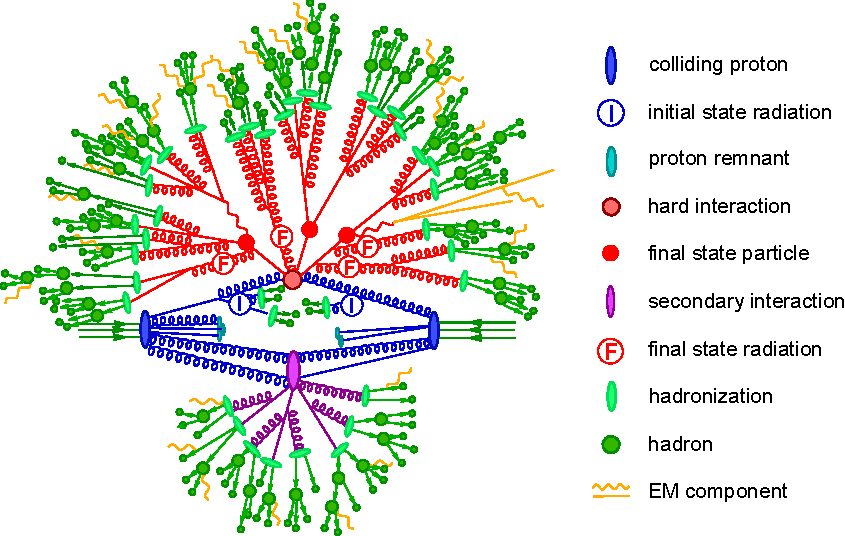
\includegraphics[scale=0.75]{figures/technique/shower.pdf}
}

A brief overview of the employed programs used for event generation and subsequent hadronization for $t$-channel single-top-quark production is given in the following.

\begin{description}
\item[MadGraph5\_aMC{@}NLO] The \MGAMC[format=hyperbf] program~\cite{Alwall:2014hca} originated from a merge of the \gls{lo} \MG[format=hyperbf] generator~\cite{Alwall:2011uj} and the \AMC[format=hyperbf] program (first showcased in Ref.~\cite{Frederix:2011zi}) into a common framework. It supports the generation of samples at \gls{lo} or \gls{nlo} accuracy together with a dedicated matching to parton showers using the \gls[format=hyperbf]{mlm}~\cite{Mangano:2006rw} or \gls[format=hyperbf]{mcatnlo}~\cite{Frixione:2002ik} schemes respectively. The latter matching scheme produces a certain fraction of events with negative weights (depending on the process) which originate from a subtraction of additional emissions from the \gls{nlo} matrix element to prevent double-counting. 
Additionally, the \MGAMC framework can produce multiple samples with additional final state partons at \gls{me} level that can be merged into a combined sample. Here, the overlap with the \gls{ps} is removed through the \gls[format=hyperbf]{mlm}~\cite{Alwall:2007fs} or \gls[format=hyperbf]{fxfx}~\cite{Frederix:2012ps} merging schemes.

\item[Powheg] The \POWHEG[format=hyperbf] box (versions~1,2)~\cite{Alioli:2010xd} is a program that contains predefined implementations of various processes such as $t$-channel single-top-quark production at \gls{nlo}~\cite{Alioli:2009je}. It utilizes the so-called \POWHEG method~\cite{Frixione:2007vw} for matching in which the hardest radiation generated from the \gls{me} has priority over subsequent \gls{ps} emissions to remove the overlap with the \gls{ps}. A small fraction of negatively weighted events may be generated in phase space regions where \gls{nlo} calculations are not feasible.

\item[CompHEP] The \COMPHEP[format=hyperbf] program (version~4.5)~\cite{Boos:2004kh} can perform calculations of cross sections from Lagrangian densities at \gls{lo}. In addition, generation of events is also possible such as single-top-quark production~\cite{Boos:2006af}. Here, an approximation is used by combining events from the $2\to2$ and $2\to3$ processes which reproduces \gls{nlo} corrections in an effective way.

\item[Tauola] Event generators can be interfaced with the \TAUOLA[format=hyperbf] library~\cite{Jadach:1993hs,Davidson:2010rw} which is specialized for simulating leptonic and hadronic decays of tau leptons with high accuracy. It accounts for spin polarization effects while the radiation of photons from \gls{qed} corrections in also included by incorporating the \PHOTOS[format=hyperbf] library~\cite{Golonka:2005pn}.

\item[MadSpin] The generation of events from processes involving the production and decay of resonances is a computational-intensive task especially at \gls{nlo}. In the narrow width approximation, where a resonant particle is taken to be on-shell, the production and decay amplitude factorizes which allows to perform the simulation of the production and decay of heavy resonances like top quarks or Higgs bosons in separate steps to reduce the complexity. The \MADSPIN[format=hyperbf] program~\cite{Artoisenet:2012st} extends this approach by also accounting for off-shell effects through a partial reweighting of events. In addition, spin correlations effects between production and decay products are taken into account as well.

\item[Pythia] The \PYTHIA[format=hyperbf] program (versions~6,8)~\cite{Sjostrand:2006za,Sjostrand:2014zea} can generate events of various processes at \gls{lo}. However, in the analyses only its famous \gls{ps} simulation is used which can be interfaced with other \gls{lo} and \gls{nlo} event generators to perform subsequent parton showering, hadronization, and the simulation of the underlying event. For hadronization, a phenomenological model is employed in which one-dimensional strings\footnote{The string model is motivated by the fact that the spatial form of a dipole color field does not extend radially like an \gls{em} field but is instead squeezed to a tube-like form.} interconnect the partons to reflect the color field. Additional partons are created through string branching which leads finally to the formation of color-neutral singlets.

\item[Herwig++] The \HERWIG[format=hyperbf] program~\cite{Bahr:2008pv,Bellm:2015jjp} is an \gls{nlo} event generator that is also capable to perform a standalone \gls{ps} simulation which can be interfaced with various other event generators as well. Similar to the usage of \PYTHIA in this thesis, only its \gls{ps} algorithm is employed for sample generation in the analyses. Its hadronization algorithm utilizes a model in which color-connected quarks are spatially kept together in clusters~\cite{Webber:1983if}. This is motivated by the concept of ``preconfinement'' for colored particles~\cite{Amati:1979fg}. If the mass of a cluster is sufficiently high it can decay into lighter clusters with a certain probability. In the final simulation step, a cluster decays then into hadrons.
\end{description}


%##############################################
\section{Top quark reconstruction}
%##############################################
\label{sec:technique-topreco}

In the presented analyses, a top quark candidate is reconstructed in data and simulated events from selected analysis objects under the assumption of $t$-channel signal top quark production. Assuming that the top quark decayed leptonically as $\mathrm{t}\to\mathrm{b}\mathrm{W}\to\mathrm{b}\ell\nu$ in selected events, its energy and momentum is calculated by summing the 4-momenta of a selected lepton candidate (muon or electron), a b-tagged jet, and a neutrino candidate. The neutrino candidate itself is reconstructed from the missing transverse momentum and the lepton momentum. By requiring a W~boson mass constraint of

\begin{align}
m_\mathrm{W}^2=\Big(80.4~\GeV\Big)^2&=\colvec{2}{E_\mathrm{W}}{\vec{p}_\mathrm{W}}^{2}\overset{!}{=}\left[\colvec{2}{E_{\ell}}{\vec{p}_{\ell}}+\colvec{2}{E_{\nu}}{\vec{p}_{\nu}}\right]^{2}\nonumber\\
&=\underbrace{m_{\ell}^2+m_{\nu}^2}_{\approx 0}+\,2\cdot E_{\ell}\,E_{\nu}-\,2\cdot\colvec{3}{p_{\ell,x}}{p_{\ell,y}}{p_{\ell,z}}\cdot\colvec{3}{p_{\nu,\mathrm{T}}\cdot\cos\phi_{\nu}}{p_{\nu,\mathrm{T}}\cdot\sin\phi_{\nu}}{p_{\nu,z}}\,, \label{eq:technique-neutrino-pz-eq}
\end{align}

where the lepton and neutrino are approximated to be massless, one can solve for the unknown $p_{\nu,z}$-component of the neutrino momentum while setting $\vec{p}_{v,\mathrm{T}}$ to the missing transverse momentum $\pvmiss$. After rearranging Eq.~\ref{eq:technique-neutrino-pz-eq}, one obtains the quadratic equation 

\begin{subequations}
\begin{align}
0&=p_{\nu,z}^2-\frac{2\,\xi\,p_{\ell,z}}{E_{\ell}^{2}-p_{\ell,z}^2}\cdot p_{\nu,z}-\frac{\xi^{2}-E_{\ell}^{2}\,p_{\nu,\mathrm{T}}^2}{E_{\ell}^{2}-p_{\ell,z}^2}\\
\xi&=\frac{m_\mathrm{W}^2}{2}+p_{\nu,\mathrm{T}}\,p_{\ell,\mathrm{T}}\cdot\cos\big(\phi_\ell-\phi_\nu\big)
\end{align}
\end{subequations}

which possesses the solutions

\begin{align}
p_{\nu,z}^{1,2}=\frac{1}{E_{\ell}^{2}-p_{\ell,z}^{2}}\left[\xi\cdot p_{\ell,z}\pm E_{\ell} \sqrt{\vphantom{\big(}\smash{\underbrace{\xi^2-p_{\nu,\mathrm{T}}^2\big(E_{\ell}^2-p_{\ell,z}^2\big)}_{\equiv \kappa}}}~\right].\vphantom{\underbrace{\Big|}_{x}} \label{eq:technique-neutrino-pz}
\end{align}

A detailed derivation of this result is given in Ref.~\cite{Chwalek:1416031}. In simulated $t$-channel single-top-quark events this procedure leads to two real solutions in about 65\% of all selected events. In Fig.~\ref{fig:technique-neutrino-reco} the difference of both real solutions with respect to the true neutrino $p_{z}$ at parton level is shown. The plot demonstrates that choosing the solution which has the smallest absolute $|p_{\nu,z}|$ value yields on average the solution which is much closer to the true neutrino $p_{z}$. Amongst the two solutions this one is the closest in about two-thirds of selected events.

\myfigure{\label{fig:technique-neutrino-reco}Difference of the reconstructed neutrino $p_{z}$ with respect to the neutrino $p_{z}$ at parton level for events with two real solutions~(distinguished by their $|p_{z}|$ value) and for events with complex solutions where the imaginary part is ignored in $t$-channel single-top-quark production.}{
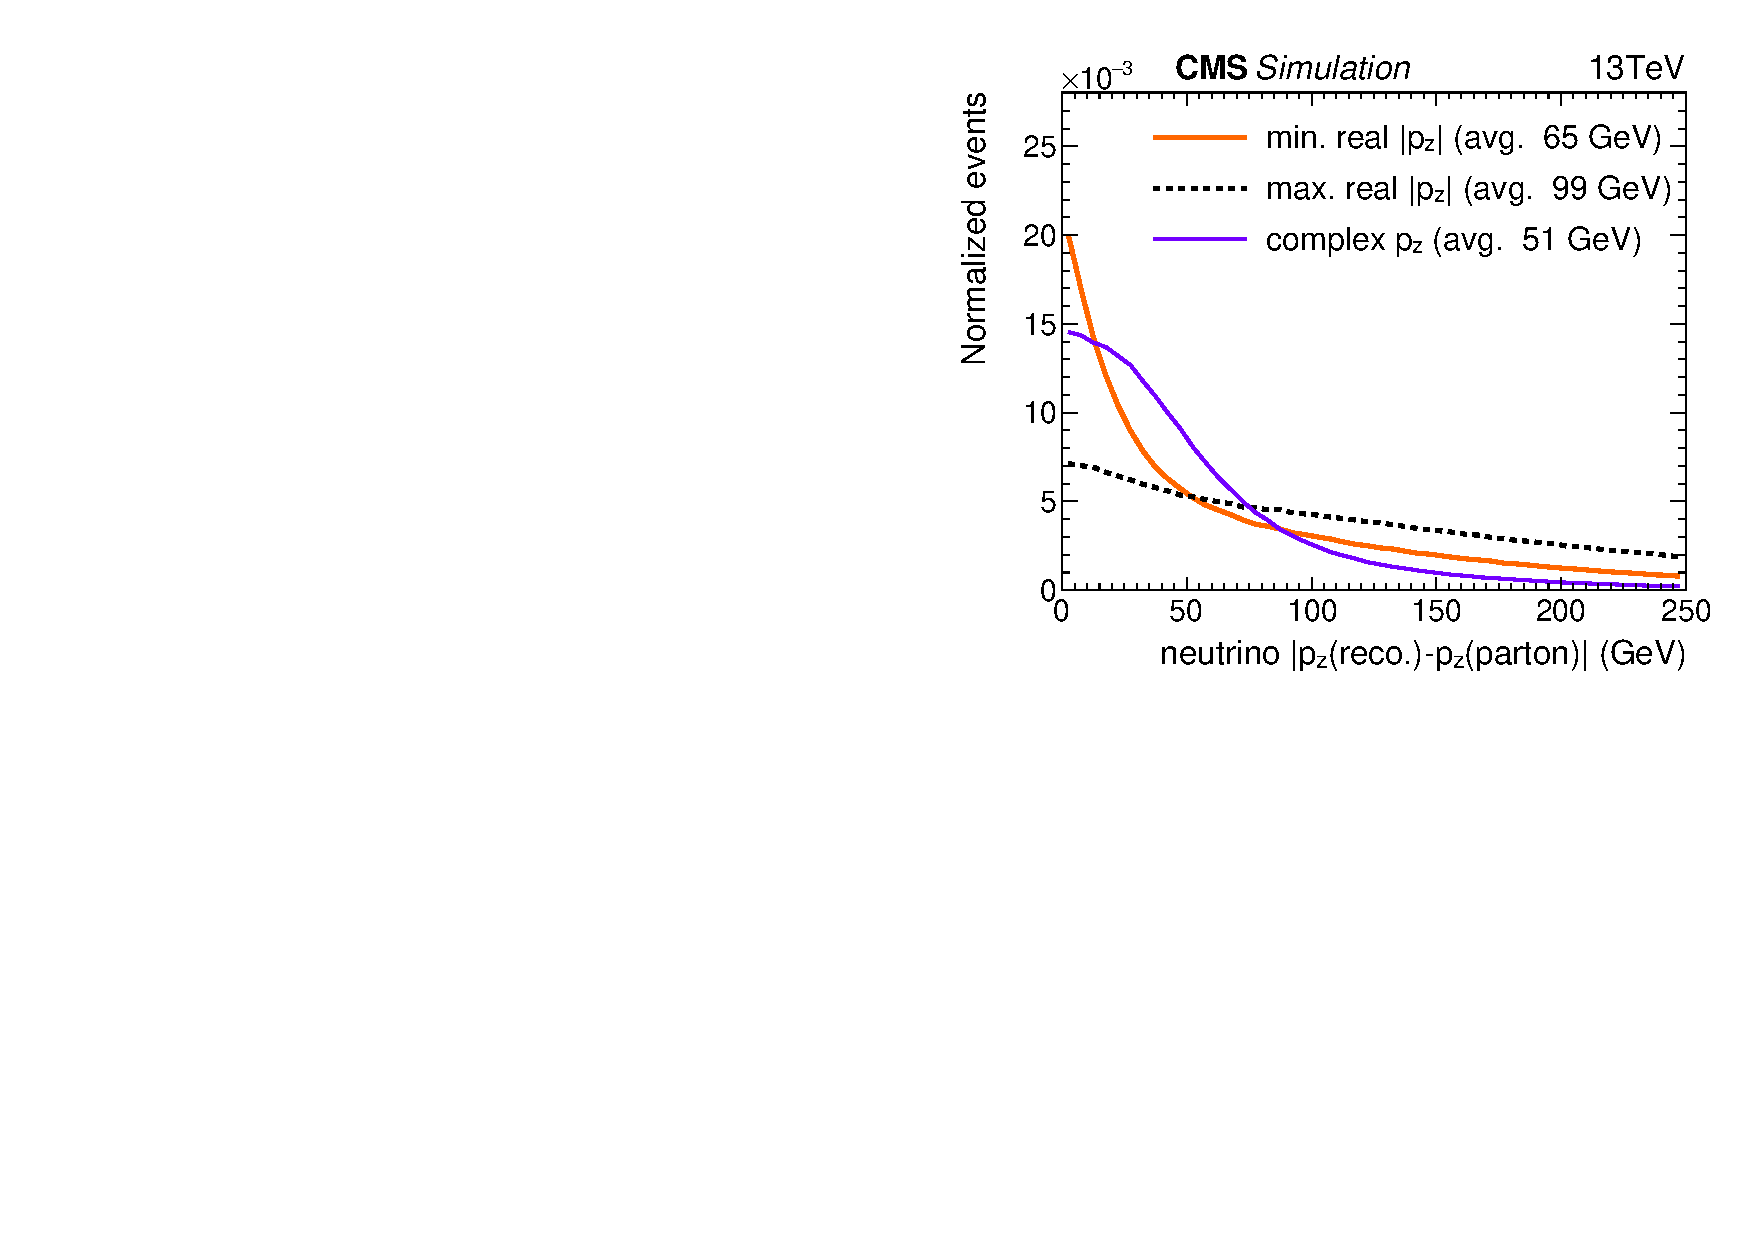
\includegraphics[width=0.52\textwidth]{figures/technique/neutrino_match_dpz.pdf}
}

Complex solutions are obtained if the radicand $\kappa$ in Eq.~\ref{eq:technique-neutrino-pz} becomes negative. This happens in about 35\% for selected signal events. Such solutions occur mostly due to the finite \met resolution whereas negligence of off-shell W~bosons and the resolution of the lepton momentum are found to be minor effects. The imaginary part of the solutions is removed by requiring that the discriminant vanishes

\begin{equation}
\kappa^{2}=\xi^2-p_{\nu,\mathrm{T}}^2\big(E_{\ell}^2-p_{\ell,z}^2\big)\overset{!}{=}0\qquad
\Rightarrow~ p_{\nu,z}=\frac{\xi\cdot p_{\ell,z}}{E_{\ell}^{2}-p_{\ell,z}^{2}}\,,\label{eq:technique-pz-complex}
\end{equation}

which is equivalent to setting the transverse mass $m_\mathrm{T}$ to the W~boson mass itself as

\begin{align}
m_\mathrm{W}^2\overset{!}{=}m_\mathrm{T}^2&=(p_{\ell,\mathrm{T}}+p_{\nu,\mathrm{T}})^2-(p_{\ell,x}+p_{\nu,x})^{2}-(p_{\ell,y}+p_{\nu,y})^{2}\nonumber\\
&\approx2\,p_{\ell,\mathrm{T}}^2\,p_{\nu,\mathrm{T}}^2\cdot\Big(1-\cos\big(\phi_\ell-\phi_\nu\big)\Big)\,.
\end{align}

\todo{check eq for mtW - units do not match!!!}

Then, the $p_{\nu,x}$ and $p_{\nu,x}$ components are varied and the pair which minimizes the distance $|\vec{p}_{\nu,\mathrm{T}}-\pvmiss|$ with respect to the measured missing transverse momentum vector is taken as the result. Figure~\ref{fig:technique-neutrino-reco} shows that after removing the imaginary part~(Eq.~\ref{eq:technique-pz-complex}) the $p_{\nu,z}$ solution is on average closer to the true neutrino $p_{\nu,z}$ momentum compared to cases with real solutions. This can be explained as follows. Initially $m_\mathrm{T}>m_\mathrm{W}$ is found in cases of complex solutions which is then modified to $m_\mathrm{T}=m_\mathrm{W}$ by ignoring the imaginary part and applying the minimization procedure as described above. One can therefore argue that this represents a correction of the missing transverse momentum which is mismeasured and thus led to the initial problem of obtaining complex solutions when solving Eq.~\ref{eq:technique-neutrino-pz}.

After finding a solution for the unknown neutrino $p_{z}$ component, a top quark candidate can be constructed. For simulated signal events, a comparison of the resulting shapes of the reconstructed top quark mass and pseudorapidity for the two neutrino solution cases is presented in Fig~\ref{fig:technique-top-reco}. For events with initial complex solutions the reconstruction procedure yields a top quark candidate with an improved mass resolution compared to events with real solutions. Similarly, the pseudorapidity of the top quark candidate demonstrates an improved reproduction of the corresponding shape at parton level as well.

\myfigure{\label{fig:technique-top-reco} Shape differences in the reconstructed top quark (a)~mass and (b)~pseudorapidity for cases with real neutrino $p_{z}$ solutions  (where the one with the smallest $|p_{z}|$ is picked) or with initially complex solutions for simulated events of $t$-channel single-top-quark production.}{
\subfloat[]{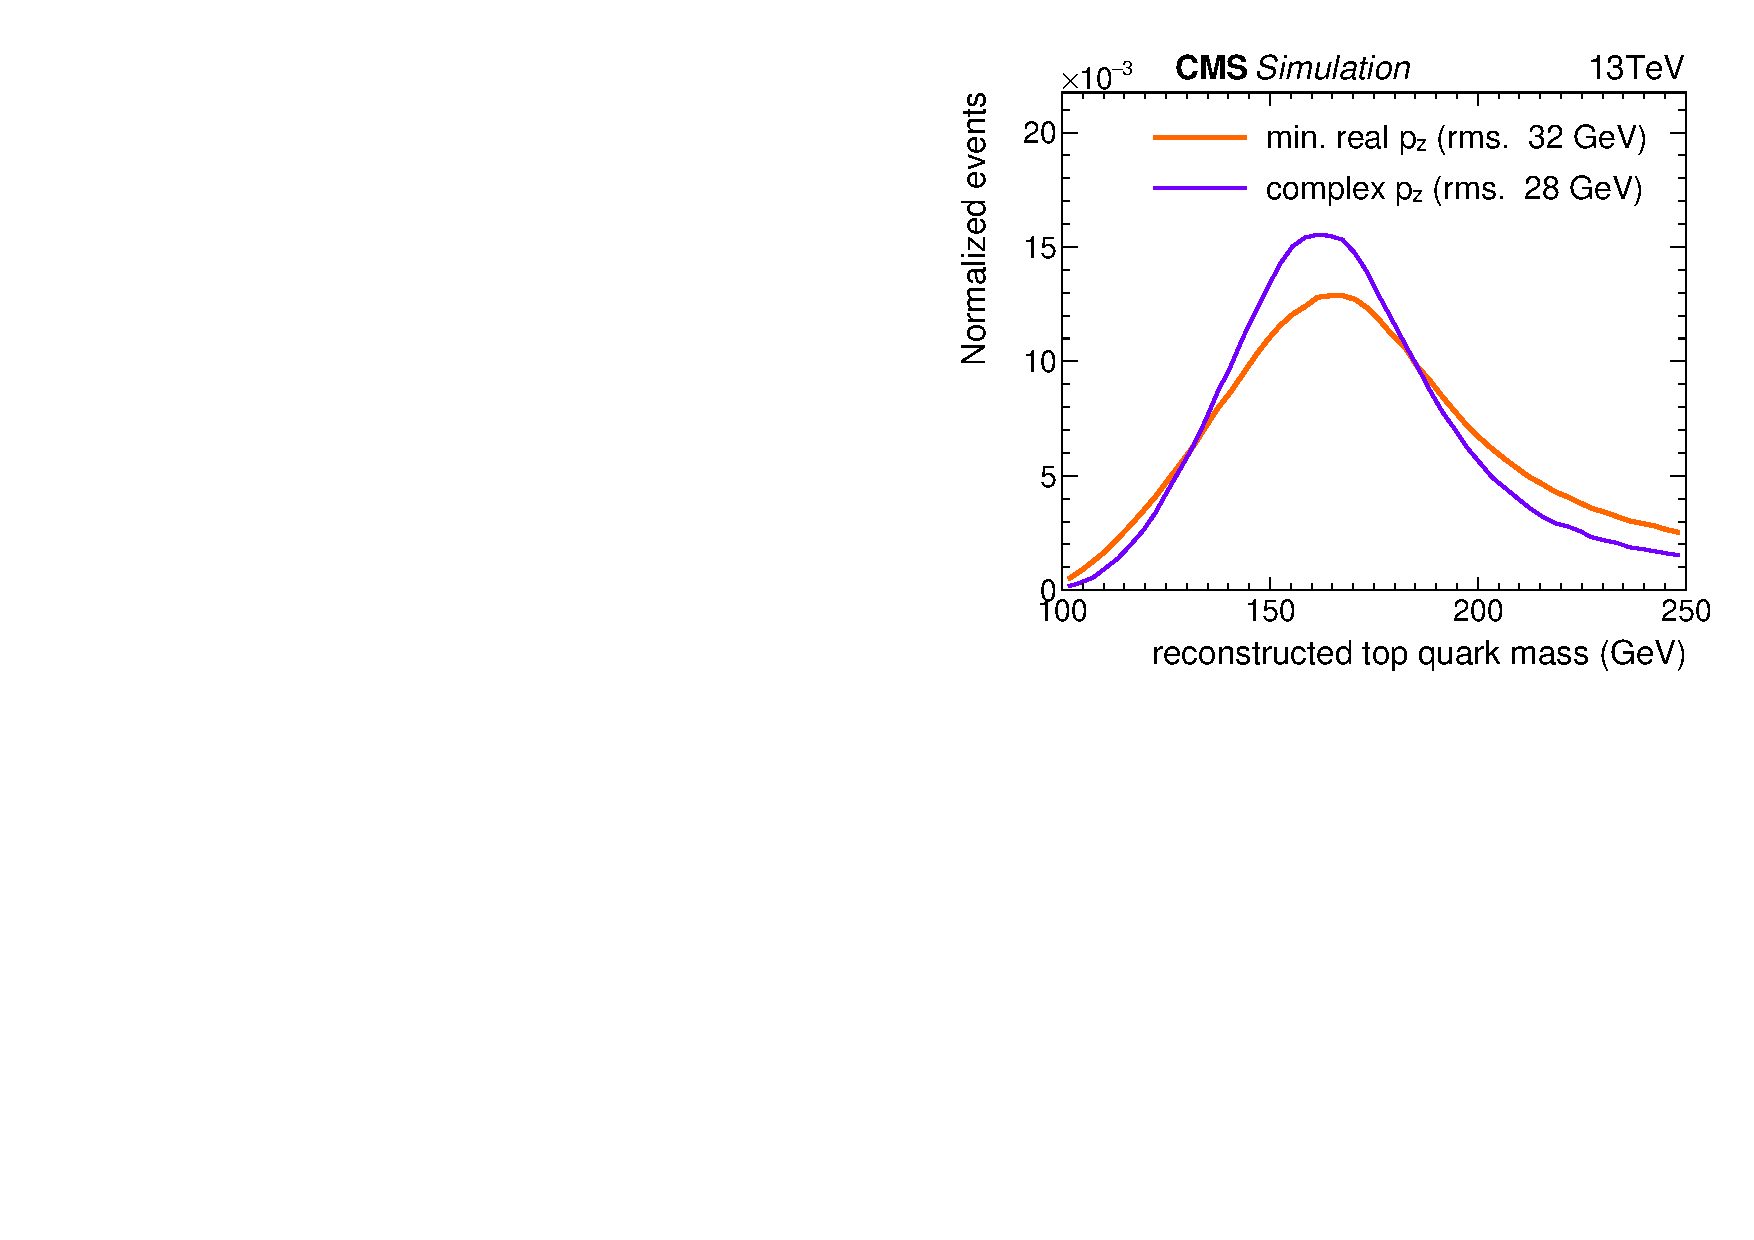
\includegraphics[width=0.48\textwidth]{figures/technique/top_match_mass.pdf}}\hspace{0.03\textwidth}
\subfloat[]{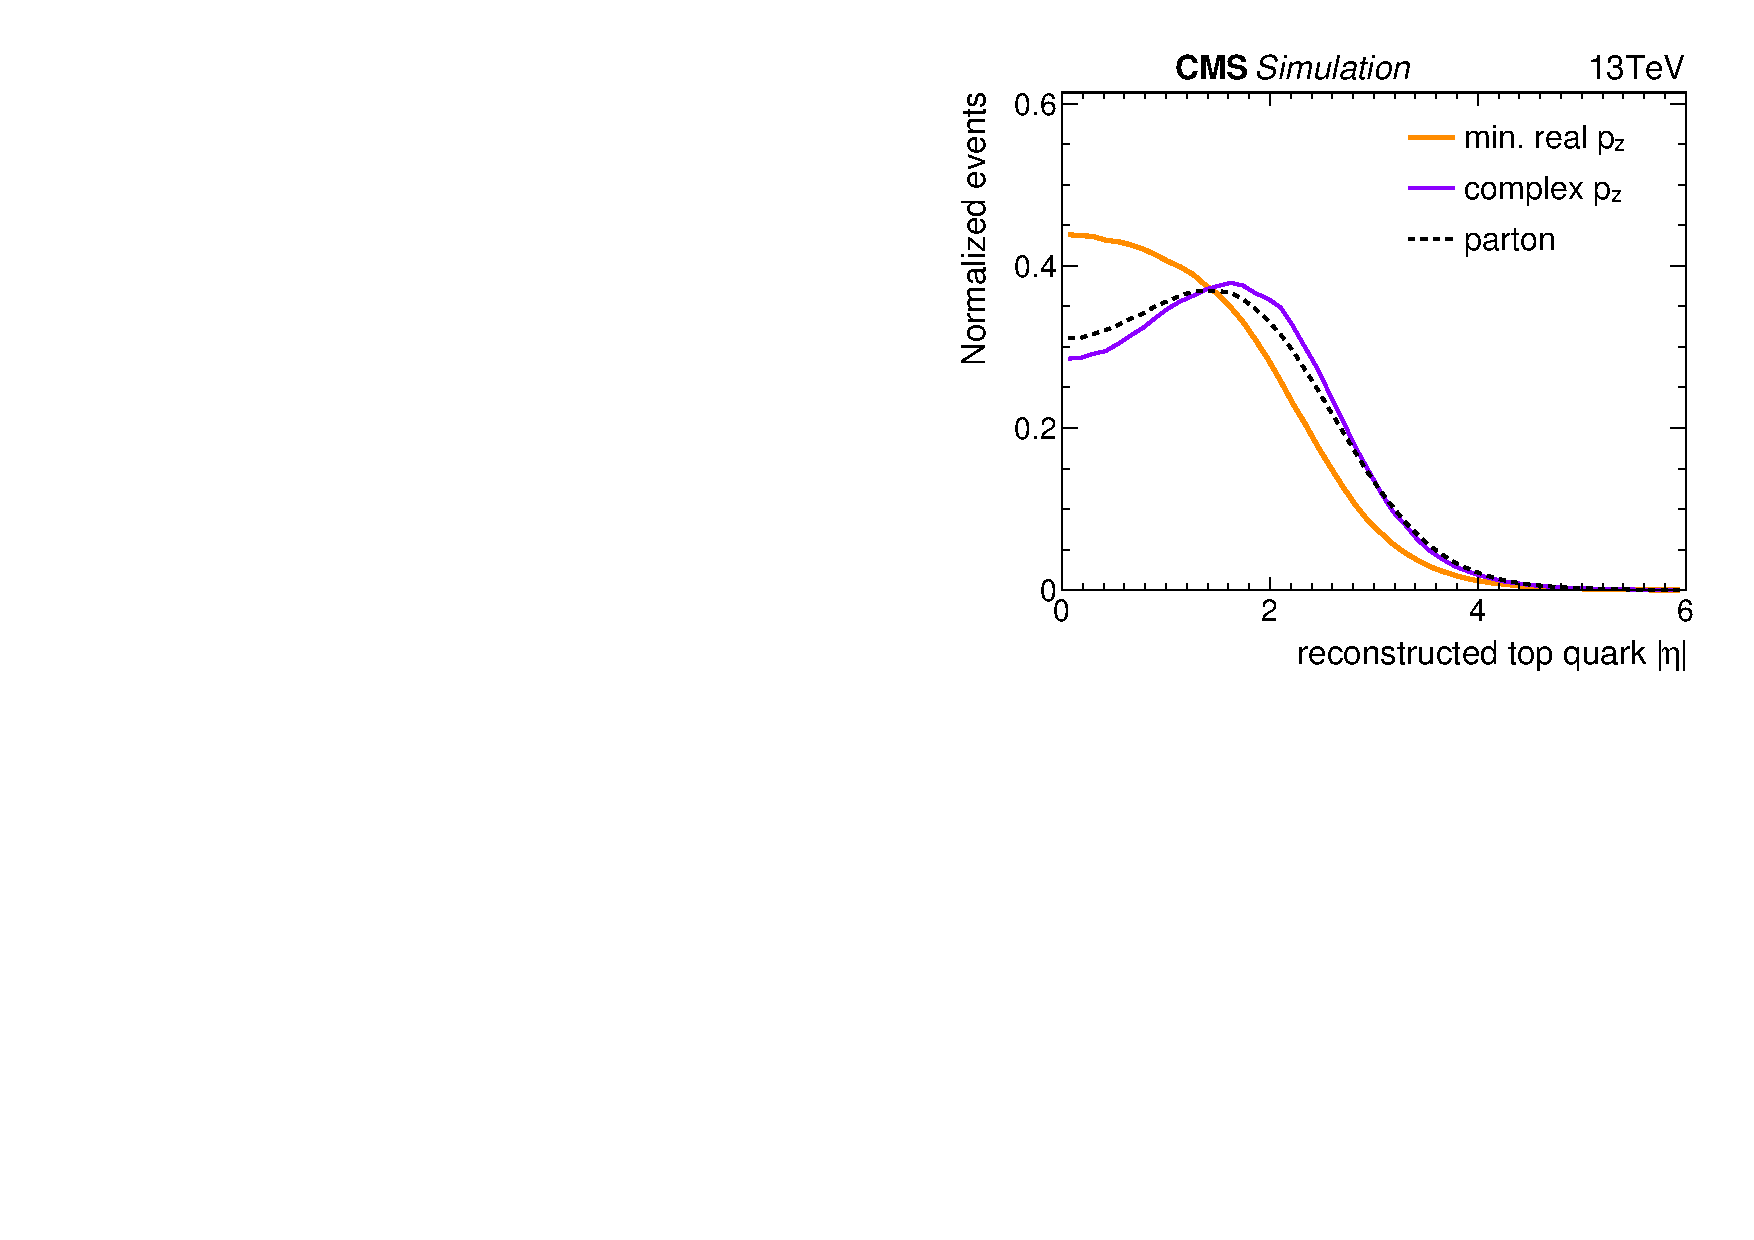
\includegraphics[width=0.48\textwidth]{figures/technique/top_match_eta.pdf}}
}


%##############################################
\section{Boosted Decision Trees}
%##############################################

After selecting data events with one isolated lepton, two jets (where one is b-tagged), and significant \met or \mtw, the majority of events does not stem from $t$-channel single-top-quark production but from background processes instead which mimic its signature. The ratios of the \glshere{sb} yields amount to about 13\% and 14\% in cross section measurements at 8~and 13~TeV, respectively~\cite{Khachatryan:2014iya,Sirunyan:2016cdg}\todo{update TOP-16-003 when accepted by PRL}.  Most of the background events stem from \wjets, \ttbar, and multijet production whereas contributions from single-top-quark production in tW and $s$~channel, \zjets, and diboson production are found to be less than 10\% at 8~TeV and 13~\TeV. The small \gls{sb} ratios motivate the usage of \glshere{mva} techniques to separate signal and background events further. In this thesis, \glsplhere{bdt} are employed for event classification as implemented in the \TMVA[format=hyperbf] framework~\cite{Hocker:2007ht}. They are based on a set of decision trees where each yields a binary output depending on whether an event is signal- or background-like. Their training and how the outputs of single decision trees are combined into a powerful one-dimensional discriminant are described in the following.

An exemplary decision tree is presented in Fig.~\ref{fig:technique-decisiontree}. It consists of sequential selections on observables $x_{i}$ which are applied on events such that the leaf nodes contain either a majority of signal or background contributions. Such trees are constructed by using samples of simulated events for which the desired classification is a priori known~(``supervised learning'').

\myfigure{\label{fig:technique-decisiontree} A sketch of a decision tree.}{
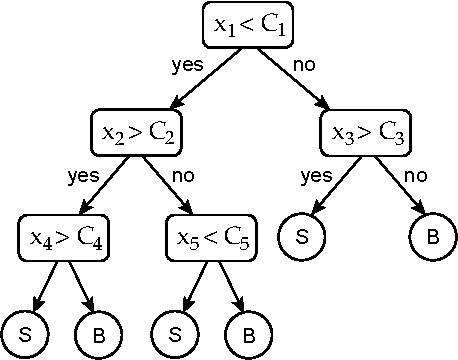
\includegraphics[scale=0.75]{figures/technique/decision_tree.pdf}
}

The optimal selection per node is found by analyzing the separation between signal and background distributions for various observables and corresponding working points $C_{i}$. In the analyses, the separation is measured as the cross entropy 

\begin{align}
H&=-p\cdot\ln(p)-(1-p)\cdot\ln(1-p)\\ p_{i}&=\frac{\int_{C_{i}}^{\infty} N_\mathrm{sig.}(x_{i})\,\mathrm{d}x_{i}}{\int_{C_{i}}^{\infty} N_\mathrm{sig.}(x_{i})+N_\mathrm{bkg.}(x_{i})\,\mathrm{d}x_{i}}\\
\Rightarrow &~\{x_{i},\,C_{i}\}=\max\Big(H\,\big|~x_{i},\,C_{i}\Big)\,,
\end{align}

where $p$ denotes the achieved purity of a selection $x_{i}>C_{i}$. Other common measures of separation in literature are the misclassification error or the so-called ``Gini'' index~\cite{Gini}. The measures are constructed to be symmetric when swapping the signal and background classes since obtaining a high purity background leaf is of equal importance for classification. A node is not split further if it contains less than a predefined minimum number of events which ensures that the decisions of all nodes and the binary output per leaf are statistically significant. This also mitigates a potential ``overtraining'' of a decision tree that occurs when statistical fluctuations are learned instead of the underlying physical distributions due to the finite statistics of the training sample.

Additional caution is required when training decision trees with a sample that contains a fraction of negatively weighted events~(e.g. generated with \MGAMC). In such cases a tree may be trained incorrectly if a significant fraction of negatively weighted events are selected in one of the nodes which are not canceled by sufficient amounts of positively weighted ones. The distributions of observables which are scanned to find the optimal node splitting can contain regions with negative yields that are unphysical. Here, the minimum number of events can be increased further beyond the statistical motivated threshold to prevent such cases. In addition, the scanned working points per observable can be preset which prevents that a decision becomes sensitive to events close to a selection border. Specifically, in the employed \TMVA framework one can configure that only a certain number of equidistantly-spaced working points are scanned per observable.
 
Single decision trees can still be affected by statistical fluctuation leading to misclassification errors when evaluated on a statistically-independent test sample. This is mitigated by training multiple decision trees with binary outputs $h_{i}\in\{-1,1\}$ which are then combined into a pseudo-continuous discriminant via a majority vote

\begin{equation}
M(\vec{x})=\sum_{i}^{N_\mathrm{trees}}~w_{i}\cdot h_{i}\,(\vec{x};\,\vec{C}_{i})\,,\label{eq:technique-majority-vote}
\end{equation}

where each decision tree output is multiplied by a weight $w_{i}$. Apart from mitigating overtraining this procedure has further advantages. It has been demonstrated in literature that the output of a majority vote can yield a classifier with high accuracy, a so-called ``strong learner'', even when all single decision trees possess only a low accuracy. In fact, it is even sufficient if the accuracy of single trees is just slightly better than random guessing~\cite{Schapire1990,FREUND1995256}. Therefore, the individual decision trees can be kept very shallow, i.e. they have only a low number of layers which also improves their robustness against overtraining. A strong learner can be obtained nonetheless by adjusting the weights in the majority vote according to the individual accuracy per tree. Usually a ``boosting'' procedure prescribes the training cycle of decision trees and how the corresponding weights have to be set.

The two boosting procedures employed in this thesis are the \ADABOOST[format=hyperbf]~\cite{FREUND1997119} (short for ``adaptive boosting'') and the \GRADIENTBOOST[format=hyperbf]~\cite{Friedman00greedyfunction} algorithms. In the \ADABOOST algorithm, decision trees are trained iteratively. At each step, a single decision tree is trained and the misclassified events are identified. Their weight is then increased in the training of subsequent trees by the boosting weight

\begin{equation}
\alpha_{n+1}=\left(\frac{1-\epsilon_{n}}{\epsilon_{n}}\right)^\beta\,,
\end{equation}

where $\epsilon_{i}$ denotes the misclassification error of the current tree $n$ and $\beta$ is a configurable learning rate. The corresponding weights in Eq.~\ref{eq:technique-majority-vote} are then given by $w_{i}=\ln\alpha_{i}$. Typically, a slow learning rate of $\beta\leq0.5$ is chosen to allow for more boosting steps. It can be shown that the \ADABOOST algorithm is equivalent to the minimization of the exponential loss function $L(M,y)=\exp(-M(\vec{x})\,y)$ where $y$ denotes the true classification of events~\cite{Hocker:2007ht}. If the loss function is instead changed to 

\begin{equation}
L(M,y)=\ln\left(1+e^{-2\,M(\vec{x})\,y}\right)
\end{equation}

the \GRADIENTBOOST algorithm is obtained. Its loss function is more robust in the presence of outliers and noise events for which the \ADABOOST algorithm may degrade. In the \GRADIENTBOOST algorithm the loss function is iteratively minimized with respect to the weights and decision tree parameters in $M$ using the method of gradient descent. During the minimization the output of the majority vote will gradually tend towards $y$ because misclassified events result in large gradients of the loss function. Similar to the \ADABOOST algorithm, an increased performance is obtained when decreasing the learning rate that controls the boosting weights which is called ``shrinkage'' here. Both boosting algorithms have been tested to validate their performances with respect to each other. Only negligible differences in their discrimination power have been found when trained on the classification problems considered in this thesis.

The discrimination power of a \gls{bdt} is assessed by analyzing the \glshere{roc} curve. Exemplary \gls{roc} curves are presented in Fig.~\ref{fig:technique-bdt-rocs} for separating $t$-channel single-top-quark events against \wjets and \ttbar background events at 13~TeV. The \glshere{auc} values denote the area under the \gls{roc} curves with respect to random guessing. They range from 0\% in case of no discrimination power to up to 50\% in the case that both event classes are fully separated in the analyzed distribution. In the figure, the \gls{roc} curves of a trained \gls{bdt} is compared to the pseudorapidity of the untagged light jet and to the reconstructed top quark mass. An \gls{auc} of about $32\%$ is achieved with the trained \gls{bdt} which outperforms the two other typical event observables for separating $t$-channel events from background processes. The exact setup of the \gls{bdt} shown here is discussed later in Sec.~\ref{sec:diff13-bdt} together with the corresponding analysis.

\myfigure{\label{fig:technique-bdt-rocs}Comparison of \gls{roc} curves for separating $t$-channel single-top-quark events from background events (\wjets and \ttbar samples mixed according to their cross section) using: random guessing; a trained \gls{bdt} discriminant; the pseudorapidity of the untagged light jet ($\jprime$); the difference between the reconstructed top quark mass and the nominal top quark mass, $|\Delta m_\mathrm{top}|=|m_\mathrm{top}^\scriptn{\mathrm{reco.}}-172.5~\GeV|$.}{
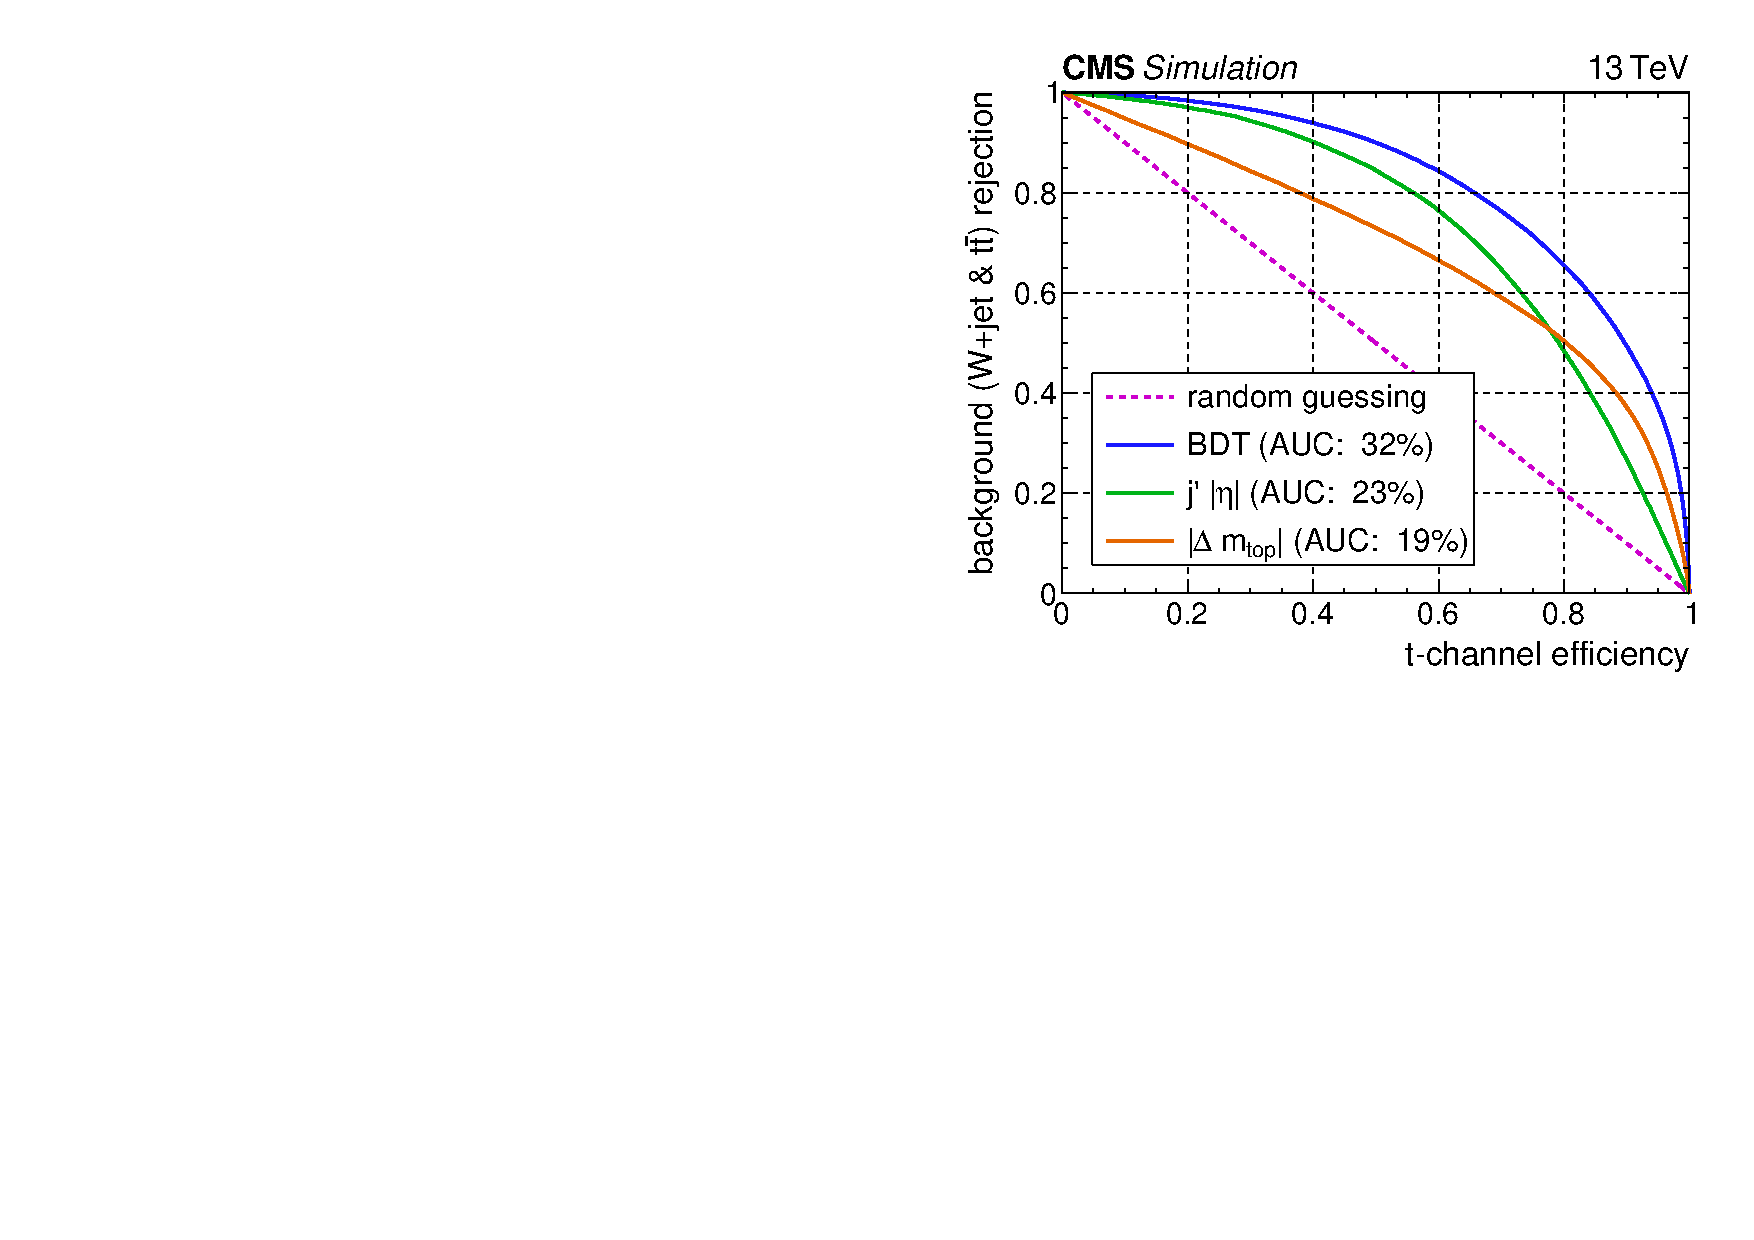
\includegraphics[width=0.5\textwidth]{figures/technique/rocs.pdf}
}


%##############################################
\section{Template-based fitting}
%##############################################
\label{sec:technique-fitting}

The amount of signal and background events in data are estimated through template-based \glshere{ml} fits. For an observable to be fitted, histograms act as templates which reflect the expected distributions of events per process. One can express the likelihood that the observed distribution in data is a realization of the  expectation as

\begin{equation}
\mathsf{L}_\mathrm{Poi.}=\prod_{i}^\mathrm{bins}~\frac{p_{i}^{\,d_{i}}\cdot e^{-p_{i}}}{d_{i}!},\qquad p_{i}=\beta^{\mathrm{(sig.)}}\cdot T^{\mathrm{(sig.)}}_{i}+\sum_{j}^\mathrm{bkgs.}~\beta^{(j)}\cdot T^{(j)}_{i} \,, \label{eq:technique-likelihood}
\end{equation}

where the amount of data events $d_{i}$ per bin $i$ is modeled as a Poisson distribution with the expected event yield $p_{i}$ as mean. The expected yields per bin are obtained by summing the signal and background templates $T^\scriptn{(X)}_{i}$. The normalization of the templates can be modified through scale factors $\beta^\scriptn{\mathrm{(X)}}$. These are then estimated from data by maximizing the likelihood. The signal scale factor is also referred to as signal ``strength'' whereas the background scale factors are sometimes called nuisance parameters because their result is of less importance. Technically, the \THETA[format=hyperbf] framework~\cite{theta} is employed for template-based fitting in this thesis where the negative logarithm of the likelihood

\begin{equation}
-\ln\Big(\mathsf{L}_\mathrm{Poi.}\big(\vec{\beta}\big)\Big)=-\sum_{i}^\mathrm{bins}~\Big[\,d_{i}\ln p_{i}\big(\vec{\beta}\big)-p_{i}\big(\vec{\beta}\big)\Big]+\mathrm{const.}
\end{equation}

is minimized instead for convenience and numerical stability. Such fits perform best when the templates feature different shapes in the fitted observable, i.e. the individual contribution to the summed expectation differs per template and additionally varies across the fitted bins. 

An estimated scale factor can be directly translated into a cross section since the templates are normalized to their expected \gls{sm} cross sections multiplied with the integrated luminosity of data. One obtains

\begin{align}
\hat{\sigma}_\mathrm{sig.}&=\frac{\hat{N}_\mathrm{sig.}}{A\cdot\epsilon\cdot{\textstyle{\int}L}}\,,\qquad
\hat{N}_\mathrm{sig.}=\hat{\beta}_\mathrm{sig.}\cdot N_\mathrm{exp.}=\hat{\beta}_\mathrm{sig.}\cdot\underbrace{\sigma_\mathrm{\gls{sm}}\cdot\textstyle{\int}L}_\mathrm{norm.}\cdot \overbrace{A \cdot \epsilon}^\mathrm{sel./reco.},\nonumber\\
&=\hat{\beta}_\mathrm{sig.}\cdot\sigma_\mathrm{\gls{sm}}\,, \label{eq:technique-xsec-measurement}
\end{align}

where $A$ denotes the acceptance and $\epsilon$ the efficiency of the event selection and reconstruction which are estimated through the simulated samples which includes also any applied corrections of the selection efficiency as summarized in Sec.~\ref{sec:reconstruction-summary}. In the fit, additional constraints are typically applied for the background scale factors by adding log-normal priors to the likelihood as

\begin{equation}
-\ln\Big(\mathsf{L}_\mathrm{total}\Big)=-\ln\Big(\mathsf{L}_\mathrm{Poi.}\big(\vec{\beta}\big)\Big)+\sum_{j}^\mathrm{bkgs.}~\frac{1}{2}\cdot\left(\frac{\ln\,\beta^{(j)}}{\delta^{(j)}}\right)^{2}\,.
\end{equation}

The additional constraints with uncertainties $\pm\delta$ reflect a priori beliefs of the background contributions in the analysis phase space where the fit is carried out. They are motivated by the fact that the selected analysis phase space is usually not optimized to measure the background yields very precisely. Log-normal distributions are explicitly preferred over Gaussian distributions for implementing these constraints because they are not biased when requiring that the scale factors have to be strictly positive. For Gaussian distributions on the other hand, such a truncation would shift their mean which can then bias the fit result.

Extra uncertainties have to be considered in the fit to account for the limited accuracy of the expected event yields per bin since the fitted templates are usually derived from samples of simulated events with finite statistics. A method proposed by R. Barlow and C. Beeston~\cite{Barlow:1993dm}, commonly called \glsmark{bb} method, introduces additional nuisance parameters $\nu_{ij}$ per bin $i$ and process $j$ which 
modify the predicted yields as $p_{i}^\prime=\sum_{j}\nu_{ij}\cdot p_{ij}$ while adding additional constraints to the likelihood which reflect the uncertainties due to the finite \gls{mc} statistics. This approach however increases the complexity of the fit due to the plethora of new parameters which have to be estimated in addition to the signal and background scale factors. The number of \gls{bb} parameters is reduced in the ``\gls{bb}-lite'' method~\cite{Conway:2011in} where the uncertainties per bin are grouped and describe by only a single nuisance parameter. A further, technical simplification can be achieved when using numerical minimization algorithms for fitting. Here, it is computationally advantageous to only maximize the likelihood with respect to the scale factors while profiling the \gls{bb} parameters per bin in each step in-situ. This approach is also implemented in the employed \THETA framework. One should note that such an approach can however result in discontinuous jumps of the likelihood. Certain minimization algorithms (e.g. \MINUIT[format=hyperbf]~\cite{James:1975dr}) may therefore not converge properly since the Hessian matrix is not positive-definite near such discontinuities. Therefore, the minimization in \THETA is explicitly set to a simple iterative Newton algorithm.



%##############################################
\section{Parton and particle level observables}
%##############################################
\label{sec:technique-levels}

Cross sections can be measured not only inclusively but also differentially in intervals of an observable. Such measurements allow to perform in-deep comparisons of data with theoretical predictions and to assess the modeling of event generators. Furthermore, some differential cross sections can be sensitive to the coupling structure of a certain process as detailed in Ch.~\ref{ch:top} and can thus be used to extract pseudo observables like the top quark spin asymmetry which is sensitive to the polarization of single top quarks produced in $t$~channel. However, to perform a proper comparison of differential cross sections, observables of interest have to be well-defined, and identical across event generators and in analytical calculations. There are two ``levels''---parton and particle level---at which physical objects of a process and related observables are typically defined.

The ``parton level'' encompasses the intermediate and final state particles within Feynman diagrams of a given process while not distinguishing between different initial states. In event generators, these partonic particles are produced in the hard interaction before hadronization. An exemplary event of $t$-channel single-top-quark production at parton level as produced by the \POWHEG event generator is shown in Fig~\ref{fig:technique-parton-example}. 

\myfigure{\label{fig:technique-parton-example}Production and decay of an exemplary $t$-channel single-top-quark event in 4~\gls{fs} at parton level as produced by \POWHEG{v2} interfaced with \MADSPIN and \PYTHIA{8}. Some intermediate state particles and vertices are not stored by the generator. Copies of particles reflecting the exclusion or inclusion of boosts induced by \gls{qcd}/\gls{qed} radiations have been omitted.}{
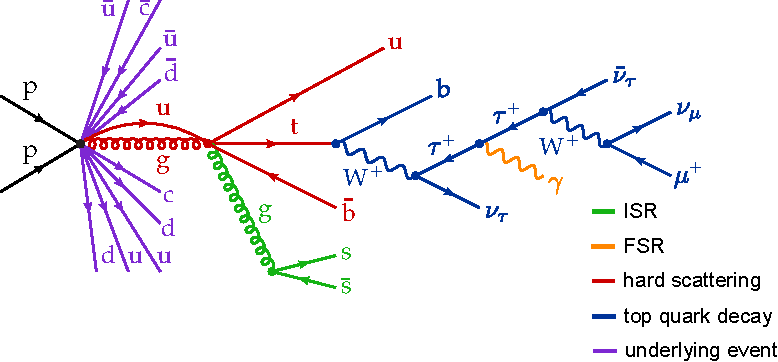
\includegraphics[scale=0.75]{figures/technique/massiveRadiation.pdf}
}

Some intermediate particles and vertices are not provided by the generator for simplicity but also due to the quantum nature of a process. Since events are generated to follow the probability of the squared sum of various matrix elements contributing to a certain process, one can usually not associate a generated event to only one specific Feynman diagram with absolute certainty. Nonetheless, various intermediate and final particles are stored unambiguously in the event record and can thus be used to define also related observables at parton level. This is detailed in the following for $t$-channel single-top-quark production.
\begin{description}
\item[Prompt charged leptons] These are charged leptons that are associated to the hard interaction and originate from the decay of a Higgs, Z or W~boson. They are thus distinguished from leptons produced in hadron decays. In $t$-channel single-top-quark production, about 15\% of the prompt muons or electrons from the top quark decay stem from an intermediate prompt tau lepton as it is for example also shown in Fig.~\ref{fig:technique-parton-example}. This fraction depends on the \pt of the muon or electron which is depicted in Fig.~\ref{fig:technique-parton-muon}. It reduces to about 6\% when requiring events with an electron or muon in the final state that has a transverse momentum of at least $20~\GeV$.
\item[Prompt neutrinos] Neutrinos are also required to be prompt and are thus associated to the hard interaction while not stemming from hadron decays. In the case of leptonically decaying tau leptons, a prompt pseudo-neutrino is defined by summing the 4-momenta of both neutrinos occurring in the decay.
\item[Top quark] The partonic top quark is required to be on-shell and to stem from the hard interaction. Some generators store multiple top quark copies in the event record which reflect different levels of the event generation process. For the analyses the top quark after accounting for \gls{qcd}/\gls{qed} radiations and the intrinsic \kt of the initial state partons is taken since it carries the most physical momentum.
\item[Spectator quark] The spectator quark occurring in $t$-channel single-top-quark production is required to be produced in association with the single top quark, i.e. they share common ancestors as depicted in Fig.~\ref{fig:technique-parton-example}. Furthermore, the spectator quark has to be a light flavored quark~(u, d, s, c) to distinguish it from a potential second b~quark occurring in 4~\gls{fs} production. At \gls{nlo}, the production of additional light quarks through \gls{isr} can lead to an ambiguity here. In such cases, the quark which balances best the top quark momentum in the transverse plane is chosen.
\end{description}

\myfigure{\label{fig:technique-parton-muon}Distributions of the (a)~transverse momentum and (b)~pseudorapidity of the final state lepton produced in $t$-channel single-top-quark production at $13~\TeV$. The lines represent various decays of W~bosons into either muons/taus directly or via intermediate tau decays. The distributions have been generated using \POWHEG{v2} interfaced with \MADSPIN and \PYTHIA{8}.}{
\subfloat[]{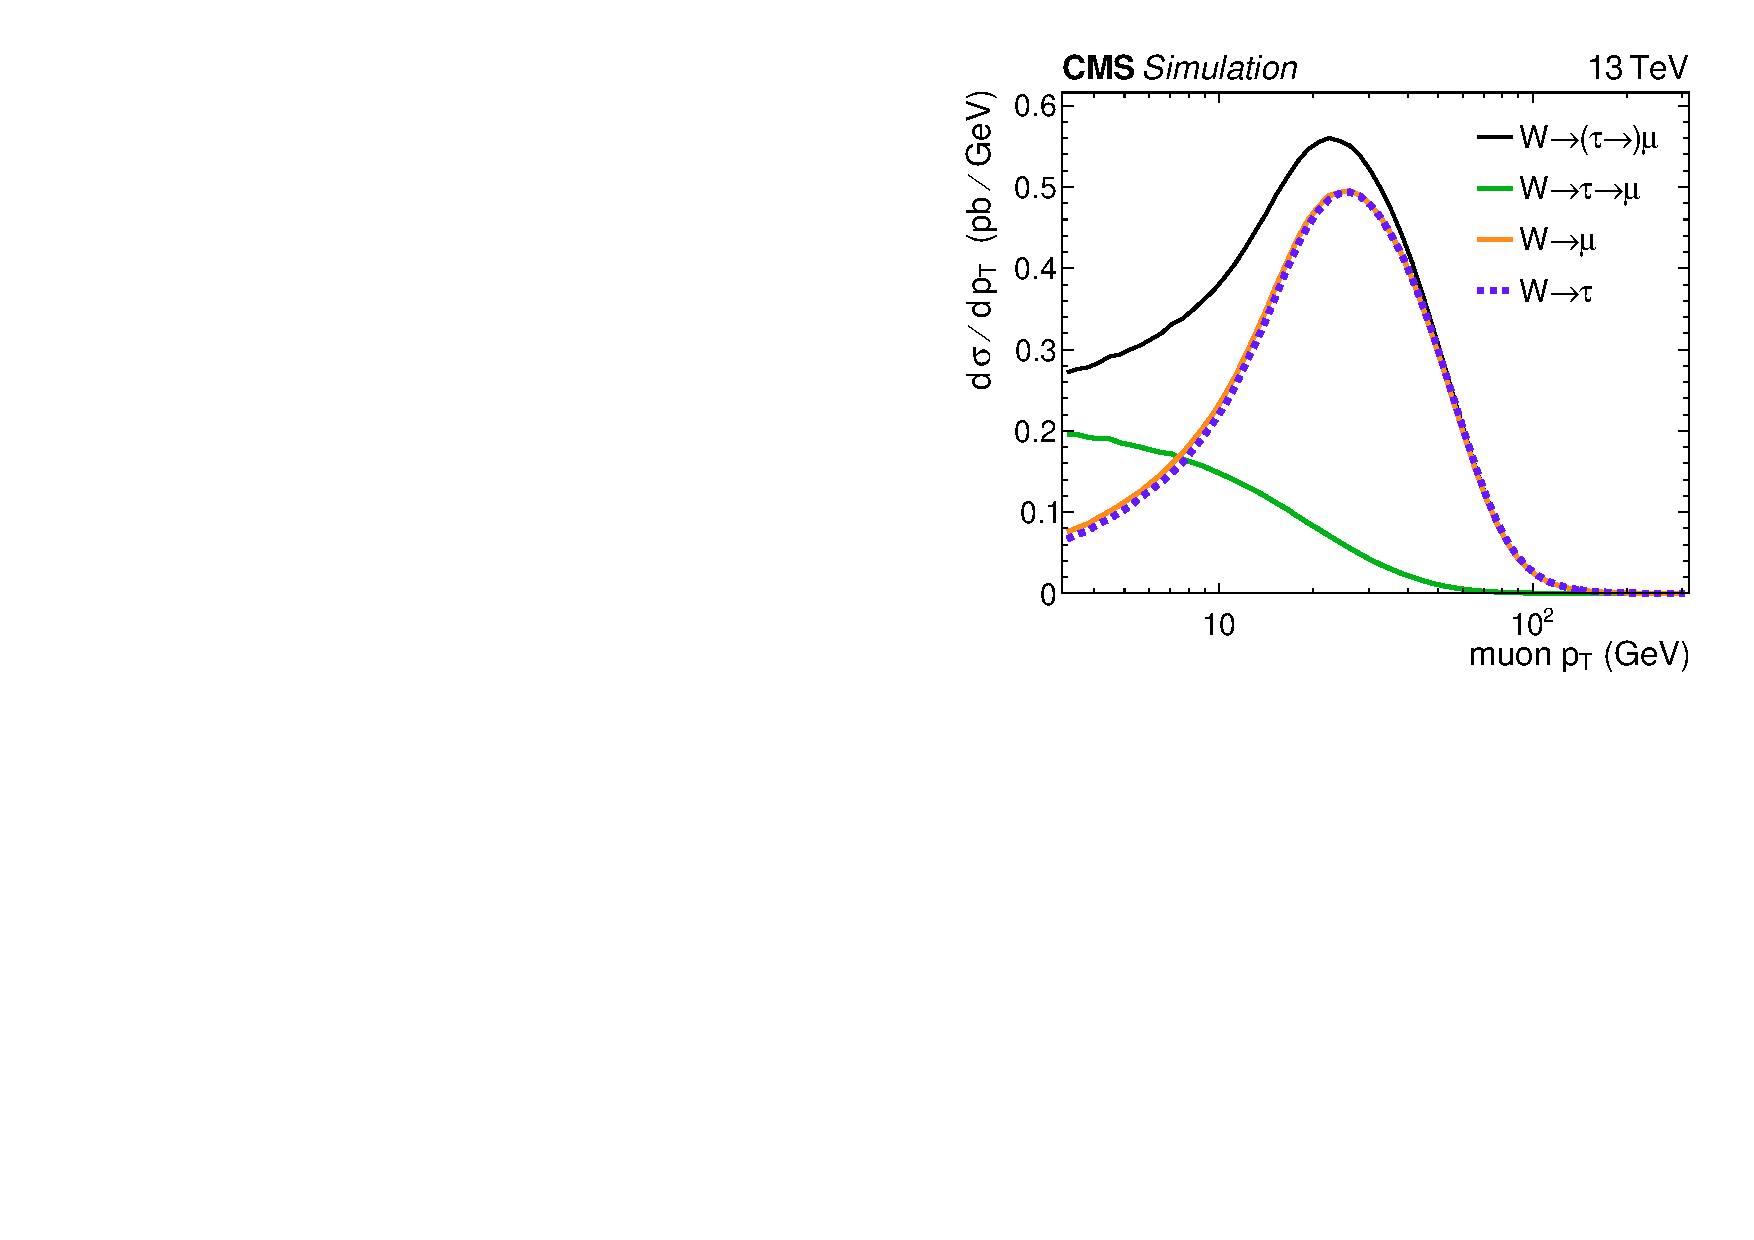
\includegraphics[width=0.48\textwidth]{figures/technique/lepton_pt.pdf}}\hspace{0.03\textwidth}
\subfloat[]{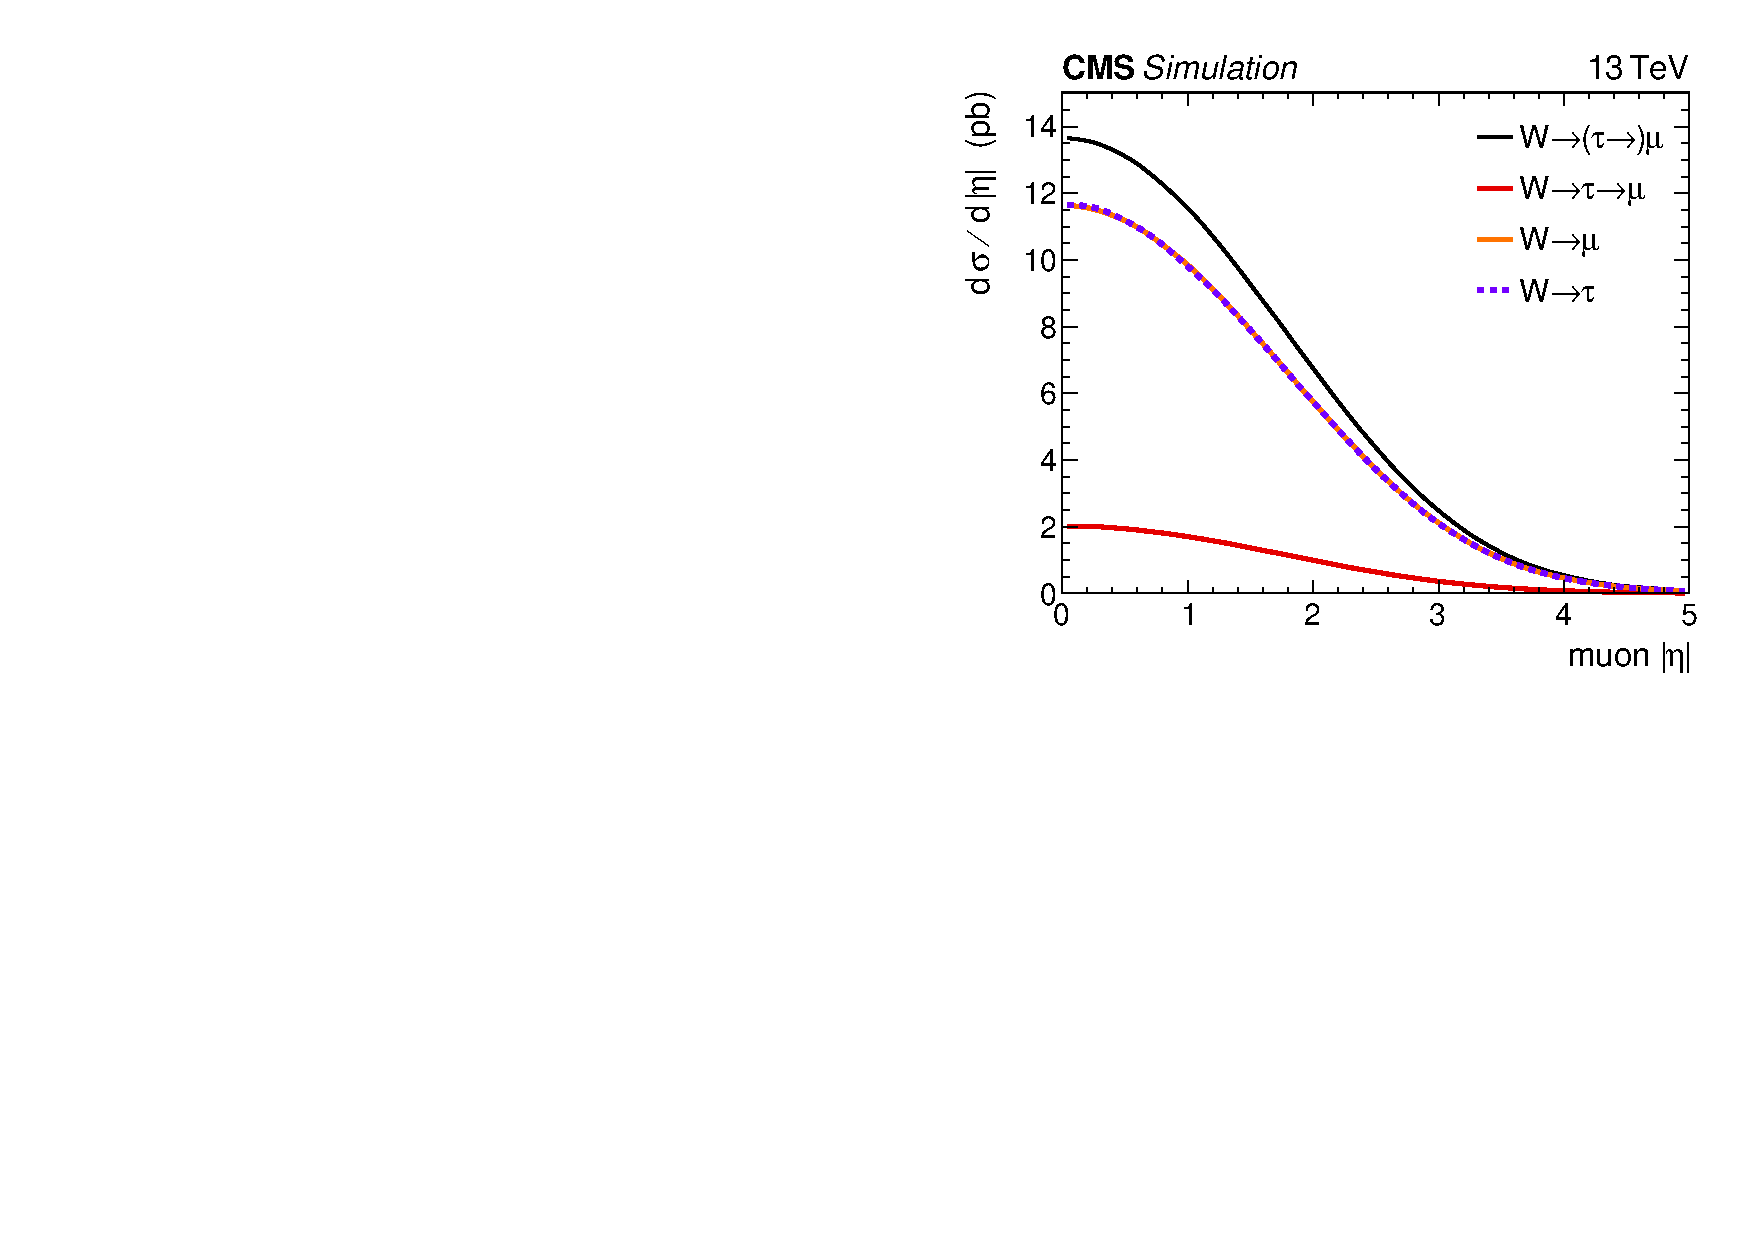
\includegraphics[width=0.48\textwidth]{figures/technique/lepton_eta.pdf}}
}

The polarization angle can be calculated from the defined objects at parton level. A comparison of its shape for the various W~boson decay chains is presented in Fig.~\ref{fig:technique-parton-cosTheta}. The $\cos\theta_{\mu}^\star$ shape is distorted when requiring events for which the lepton momentum is above a certain threshold. This results into a drop of the distribution at $\cos\theta^{*}_{\mu}\to 1$ which is demonstrated in Fig.~\ref{fig:technique-parton-cosTheta20} where the polarization angle is shown for events with $\pt(\mu)>20~\GeV$ only.

\myfigure{\label{fig:technique-parton-cosTheta}Distributions of the polarization angle for $t$-channel single-top-quark production at $13~\TeV$: (a)~inclusive distribution; (b)~only events with $\pt(\mu)>20~\GeV$. The lines represent various decays of W~bosons into either muons/taus directly or via intermediate tau decays. The distributions have been generated using \POWHEG{v2} interfaced with \MADSPIN and \PYTHIA{8}.}{
\subfloat[]{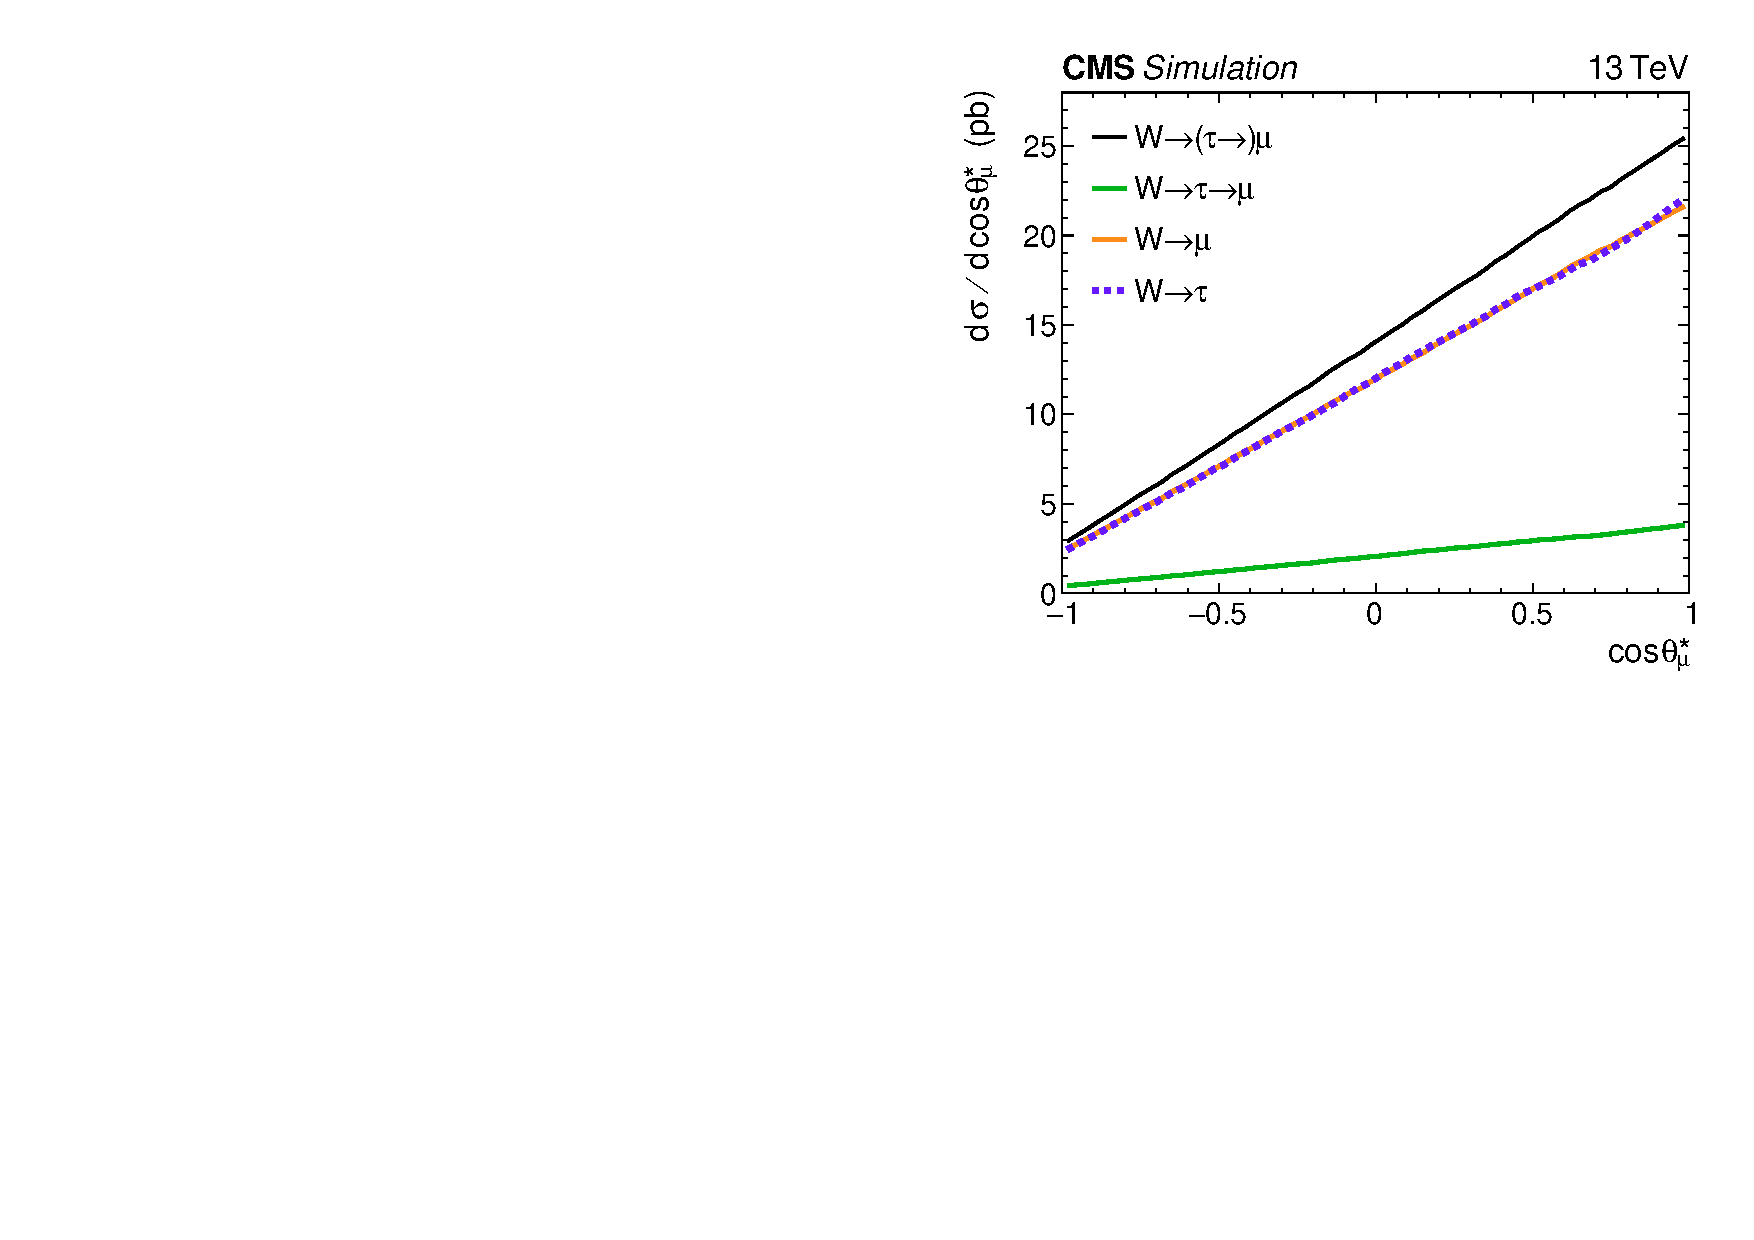
\includegraphics[width=0.48\textwidth]{figures/technique/cosTheta.pdf}}\hspace{0.03\textwidth}
\subfloat[\label{fig:technique-parton-cosTheta20}]{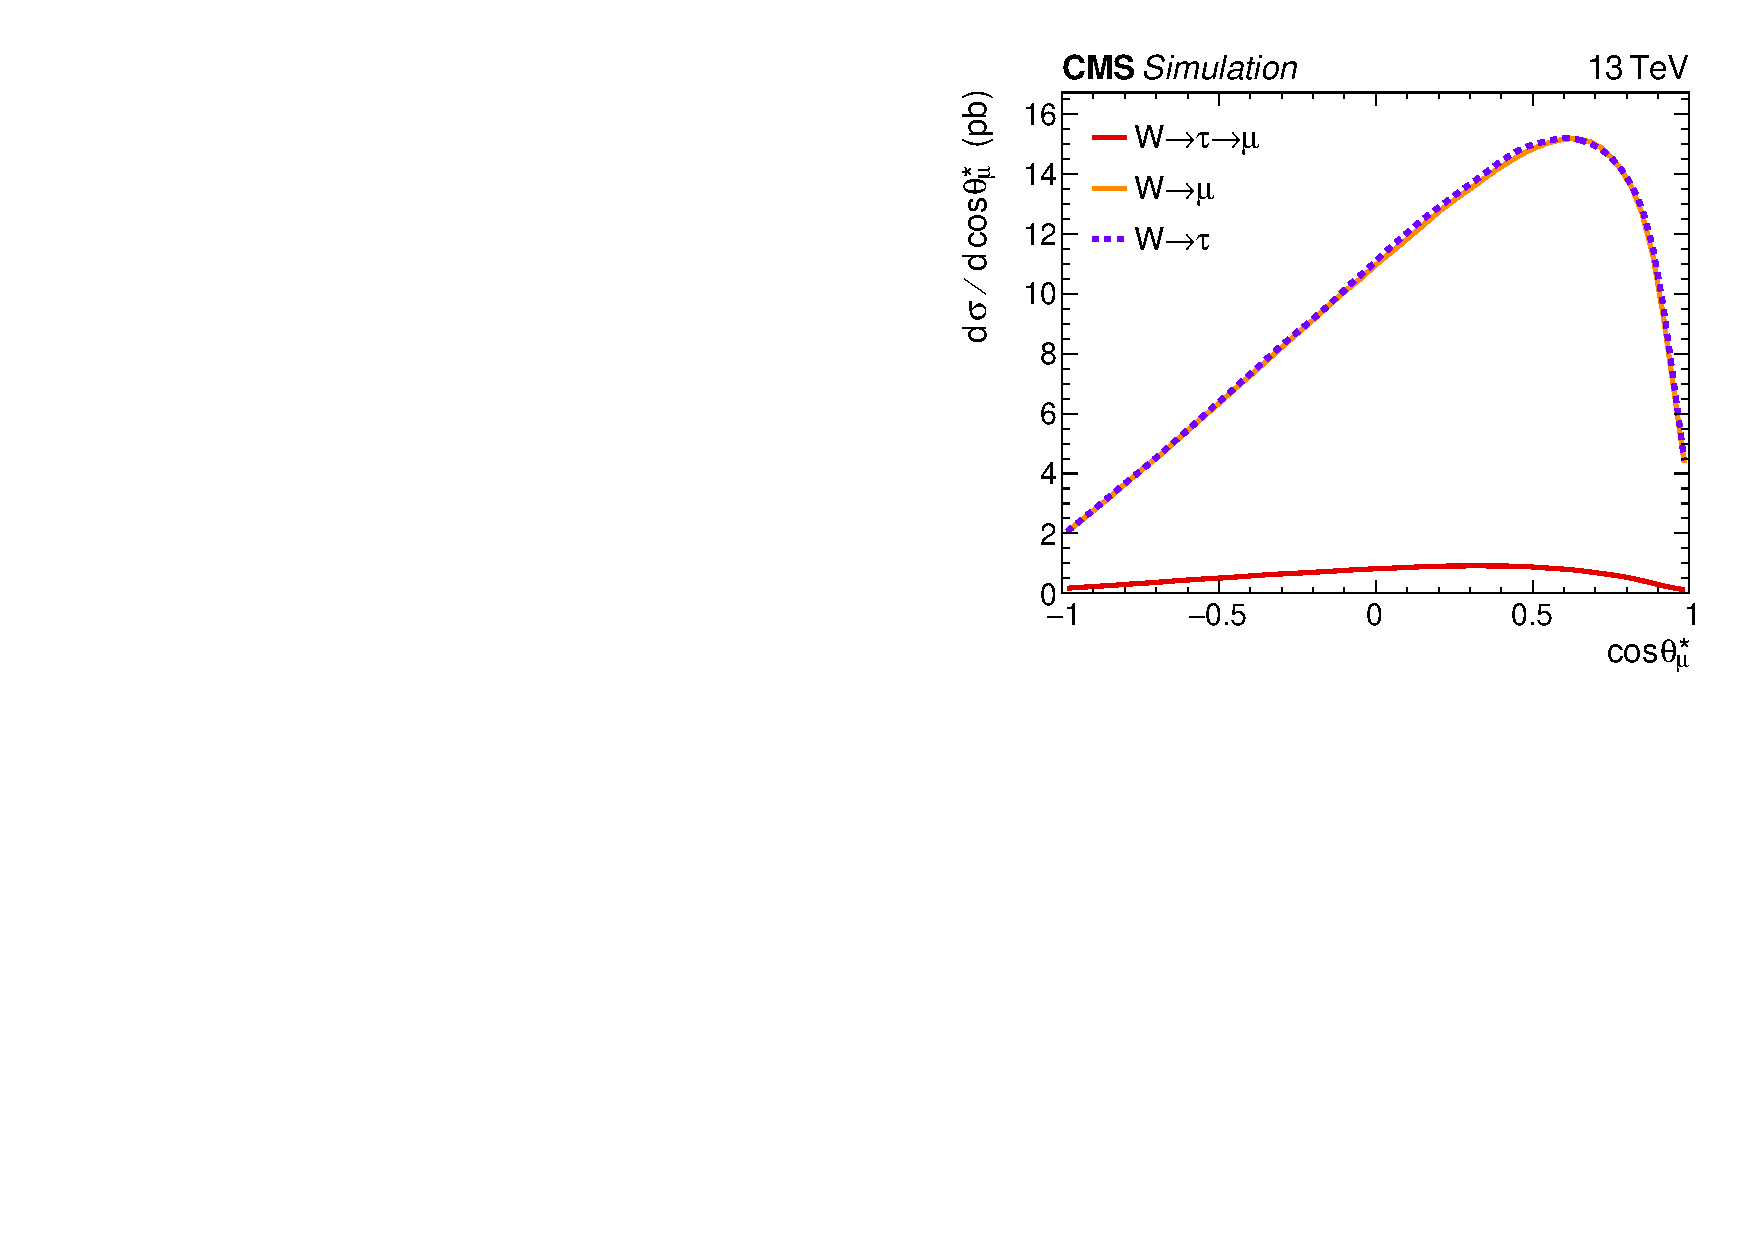
\includegraphics[width=0.48\textwidth]{figures/technique/cosTheta_lpt20.pdf}}
}

Another level at which observables can be defined is the ``particle level''. Here, an event selection similar to the one at reconstruction level is applied on the generated particles after hadronization. This allows to report results close to the ``fiducial'' phase space of the detector. The advantage is that an extrapolation into the inclusive phase space as it is intrinsically performed for parton level measurements (e.g. inclusive cross sections) is not required. A sketch of parton and particle level objects for $t$-channel single-top-quark production and their correspondence is depicted in Fig.~\ref{fig:technique-parton-particle}. Objects at particle level are defined by utilizing only the final particles produced by event generators and subsequent parton showers which have a mean lifetime of more than $30~\mathrm{ps}$ and are therefore considered to be stable. Final state quarks and gluons appear as jets after hadronization which consist of hadrons and non-prompt leptons. Charged leptons may radiate photons which are accounted for by clustering them with close-by photons. These are then referred to as ``dressed'' leptons. The performed clustering yields a universal treatment of \gls{qcd}/\gls{qed} radiations without relying on information about intermediate particles in the decay chain which is more complicated at parton level (especially for the definition of the spectator quark in the case of \gls{fsr} as for example demonstrated in Fig.~\ref{fig:technique-parton-particle}). Detailed definitions of the analysis objects at particle level used in this thesis are provided in the following.

\myfigure{\label{fig:technique-parton-particle}A sketch of parton and particle level objects in $t$-channel single-top-quark production. An additional gluon has been added as a final state radiation.}{
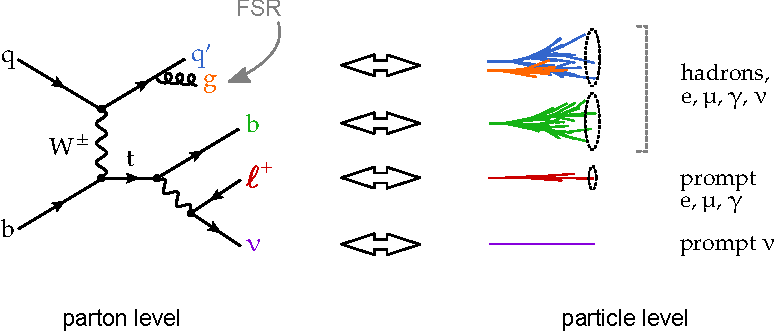
\includegraphics[scale=0.75]{figures/technique/fiducial.pdf}
}

\begin{description}
\item[Dressed leptons] Photons which do not stem from hadron decays are clustered with prompt muons or electrons if they are within $\Delta R=\sqrt{\Delta\eta^2+\Delta\phi^2}<0.1$. A dressed lepton consists of exactly one charged lepton and any number of potentially close-by photons.
\item[Neutrinos] The 4-momenta of all prompt neutrinos are summed to define the missing transverse energy. To improve the agreement with the neutrino candidate at reconstruction level, the same algorithm as described in Sec.~\ref{sec:technique-topreco} is applied at particle level using a dressed lepton here to solve for the neutrino $p_{z}$ component.
\item[Jets] Jet are clustered from stable particles excluding all neutrinos and the particles used to define the dressed leptons. The anti-$k_\mathrm{T}$ algorithm with a distance of $R=0.4$ is employed at 13~TeV copying the jet size at reconstruction level. The ``ghost'' b-tagging method~\cite{Cacciari:2008gn} where jets are tagged by using B-hadrons with rescaled momentum will not be utilized here since its high efficiency is found to disagree with the performance of the tagging algorithm at reconstruction level. More details will be discussed in Ch.~\ref{ch:prospects}.
\item[Pseudo top quark] A pseudo top quark is reconstructed by combining the 4-momenta of a dressed lepton, a neutrino candidate, and a jet. Since the ghost b-tagging method is not utilized, the jet which yields a top quark mass that is closest to $172.5~\GeV$ is chosen in the pseudo top quark reconstruction.
\end{description}

After applying a suitable selection on the particle level objects, the fiducial cross section can obtained by modifying Eq.~\ref{eq:technique-xsec-measurement} as

\begin{equation}
\sigma_\mathrm{sig.}^\mathrm{fid.}=\frac{N_\mathrm{sig.}\cdot A_\mathrm{fid.}}{A_\mathrm{reco.}\cdot\epsilon_\mathrm{reco.}\cdot{\textstyle{\int}L}} =\sigma_\mathrm{sig.}^\mathrm{inc.}\cdot A_\mathrm{fid.}\,,
\end{equation}

where $A_\mathrm{fid.}$ denotes the acceptance of events in the fiducial phase space. Similar to the acceptance and efficiency of the event selection at reconstruction level, it can be estimated from a sample of simulated signal events as $A_\mathrm{fid.}=N_\mathrm{fid.}/N_\mathrm{total}$. 



%##############################################
\section{Unfolding}
%##############################################

Distributions of reconstructed data events are typically distorted due to finite resolution, acceptance, and reconstruction inefficiencies of the detector with respect to the parton or particle level. The idea of unfolding in \gls{hep} is to ``revert'' these effects. An unfolded distribution can then easily be compared to the expectations from theory or to equivalent measurements. A reconstructed distribution can be modeled as

\begin{equation}
\underbrace{~f(y)~}_\mathrm{reco.}=\int \underbrace{A(y)\,\epsilon(y)\, R(y,x)}_\mathrm{detector}~~\cdot \underbrace{~g(x)~}_\mathrm{true}\, \mathrm{d}x\,, \label{eq:technique-fredholm}
\end{equation}

where a true distribution $g(x)$ of interest (i.e. at parton or particle level) is folded with the detector response $R(y,x)$ times the acceptance of the event selection $A(y)$ and the reconstruction efficiency $\epsilon(y)$. Mathematically, Eq.~\ref{eq:technique-fredholm} is called a Fredholm equation of first kind. Unfolding is then a procedure to estimate the true distribution given $f(y)$, $A(y)$, $\epsilon(y)$, and $R(y,x)$. 

Equation~\ref{eq:technique-fredholm} can be discretized and written as a matrix equation

\begin{equation}
\vec{y} = \widetilde{\mathcal{R}}\cdot\vec{x}\,,\qquad \widetilde{\mathcal{R}}=\mathcal{A}\cdot\mathcal{E}\cdot\mathcal{R}\,, \label{eq:technique-folding}
\end{equation}

where the continuous distributions are converted into vectors~(histograms) and the response, acceptance, and efficiency functions are described by matrices~(two-dimensional histograms). Elements of the response matrix $\mathcal{R}_{ij}$ can be interpreted as the transition probability $p_{i\to j}$ that an observable in bin $i$ at truth level is measured in bin $j$ by the detector. Attempting to solve Eq.~\ref{eq:technique-folding} for $\vec{x}$ through a simple inversion of the response matrix reveals that the unfolding problem is actually ill-posed. A simple inversion can result in unstable solutions with large variances and significant anticorrelations between bins. Figure~\ref{fig:technique-ill-unfolding} demonstrates this for a simple model which is defined as

\begin{subequations}\label{eq:technique-unfolding-test-model}
\begin{align}
g(x)&=\frac{1}{2}+A\cdot x\,,\qquad A=0.44\\
R(y,x)&\propto\mathrm{exp}\left(\frac{1}{2}\cdot\frac{(x-y)^2}{\sigma^2}\right)\,,\qquad \sigma=0.15\,.
\end{align}
\end{subequations}

Here, a distribution $g$, similar to the expected distribution of the top-quark polarization angle at parton level, has been folded with a simple Gaussian smearing function $R$. When unfolding by inverting the response matrix, a small deviation~(dash-orange line) from the folded distribution~(violet markers) results into an unphysical, oscillating solution due to the introduced anticorrelations.

\myfigure{\label{fig:technique-ill-unfolding}Exemplary unfolding of a distribution using a simple inversion of the response matrix: (a)~true distribution with overlaid unfolding results; (b)~the true distribution after folding and a sample of a corresponding statistical fluctuation.}{
\subfloat[\label{fig:technique-ill-unfolding-true}]{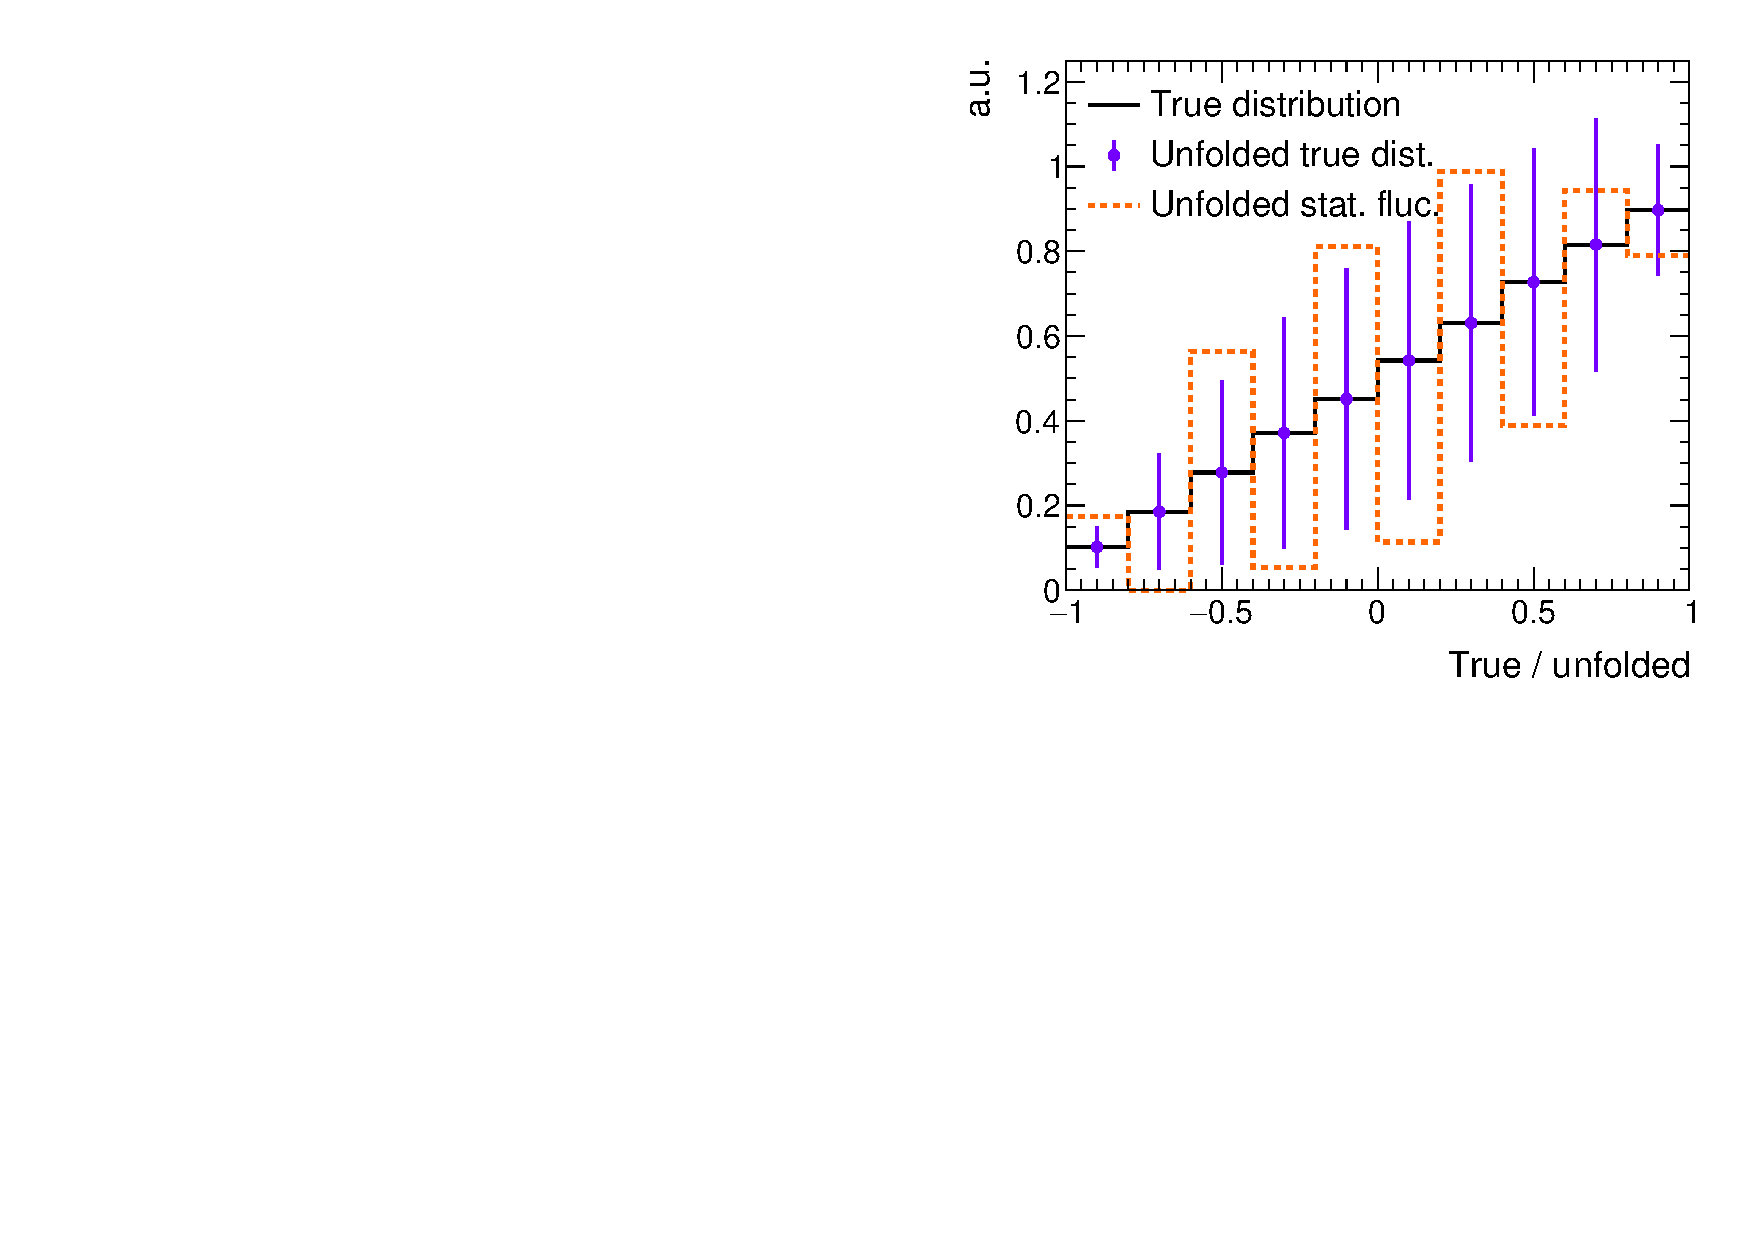
\includegraphics[width=0.48\textwidth]{figures/technique/trueDist.pdf}}\hspace{0.03\textwidth}
\subfloat[\label{fig:technique-ill-unfolding-reco}]{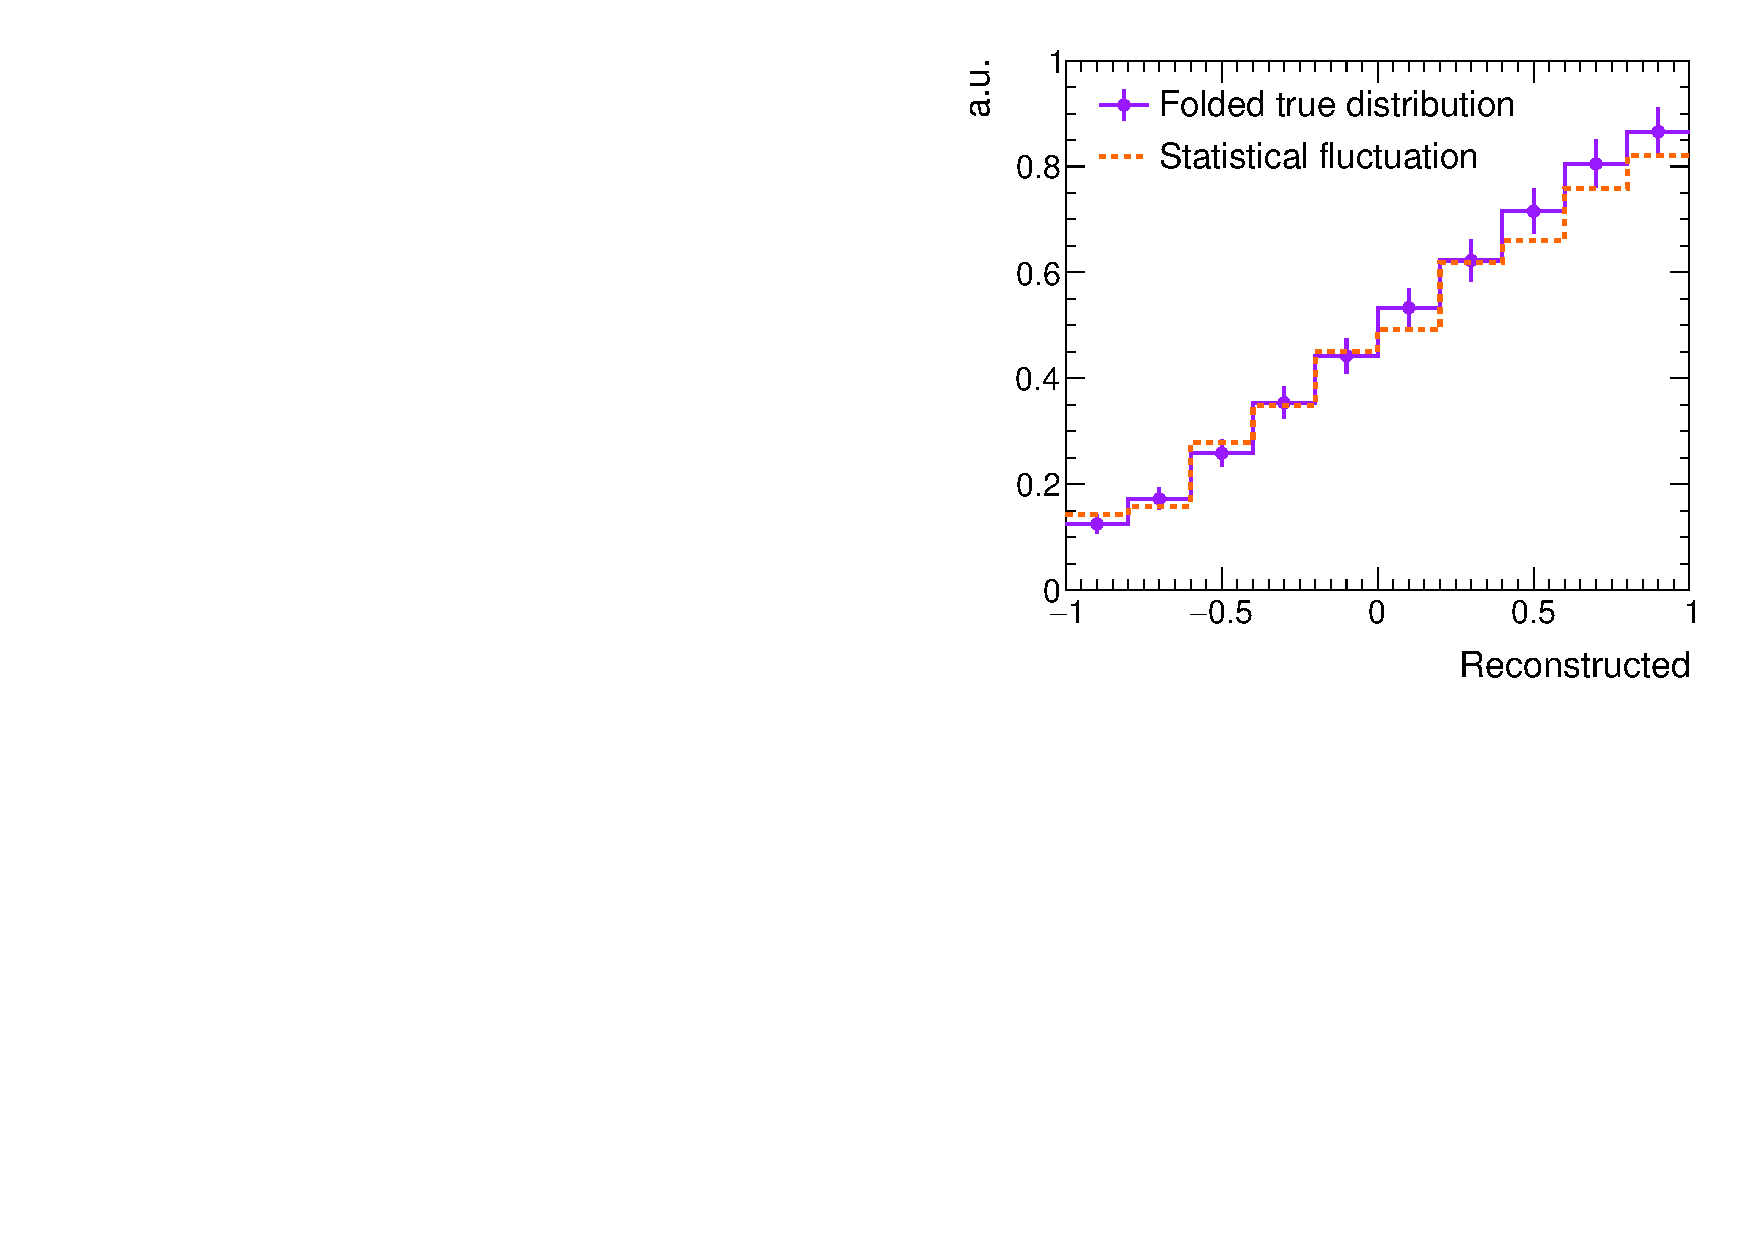
\includegraphics[width=0.48\textwidth]{figures/technique/recoDist.pdf}}
}


The origin of these oscillations can be investigated by performing a \glshere{svd} of the unfolding problem~(Eq.~\ref{eq:technique-folding}). The \gls{svd} is a generalization of the eigendecomposition that allows to decompose even non-quadratic matrices as 

\begin{equation}
\vec{x}=\Big(\widetilde{\mathcal{R}}\Big)^{-1}\vec{y}\\
=\Big(\mathcal{U}~\cdot\underbrace{\mathcal{S}}_\mathrm{diagonal}\cdot~\mathcal{V}\Big)^{-1}\vec{y}~=~\mathcal{V}^{-1}\cdot
\begin{tikzpicture}[baseline=(current bounding box.center),every left delimiter/.style={xshift=0.4em},every right delimiter/.style={xshift=-.4em},]
\matrix (m) [matrix of math nodes,nodes in empty cells,row sep=-1.5mm,left delimiter=(,right delimiter={)},inner sep=0pt,nodes={inner sep=.3333em},]{
\frac{1}{s_{11}} &  & 0  \\
0 & & \frac{1}{s_{nn}} \\
} ;
\draw[dotted,thick] (m-1-1)-- (m-2-3);
\end{tikzpicture}
\cdot~~\mathcal{U}^{-1}~\vec{y}\,,
\end{equation}


where $\mathcal{U}$ and $\mathcal{V}$ contain the so-called left- and right-singular vectors, respectively. The matrix $\mathcal{S}$ has only non-zero elements $s_{ii}$ on its diagonal which are also referred to as singular values. Typically, they are ordered as $s_{ii}>s_{i+1,i+1}$ while the singular vectors are normalized to $1$. The vectors are orthogonal to each other and can be interpreted as modes of the measured distribution. When a singular value is small, the unfolded distribution becomes unstable since the corresponding mode in the reconstructed distribution is unphysically amplified by $1/s_{ii}$ through the inversion.

Various regularization procedures have been proposed to mitigate this problem. The most straightforward regularization scheme is utilized in the ``\gls{svd} unfolding'' algorithm~\cite{Hocker:1995kb}. Here, the response matrix is modified as

\begin{equation}
\Big(\mathcal{R}^\mathrm{reg.}[\tau]\Big)^{-1}_{ ij}=\sum_{k}^{\tau}~\mathcal{V}^{-1}_{ik}\cdot\left(\frac{1}{s_{kk}}\right)\cdot~\mathcal{U}^{-1}_{kj}\,,
\end{equation}

where the regularization parameter $\tau$ controls a cutoff that keeps only singular values with indices $k\leq\tau<n$ during the inversion. Thus, higher order modes in the reconstructed distribution leading to oscillating solutions are ignored. A more sophisticated unfolding method can be derived from the Tikhonov regularization scheme~\cite{Tikhonov}. Here, the unfolding problem~(Eq.~\ref{eq:technique-folding}) is rewritten as a minimization of the loss function

\begin{align}
L\big(\vec{x}\big)&=\big|\big|\,\vec{y}-\tilde{\mathcal{R}}\cdot\vec{x} \,\big|\big|^{2}~+~~\big|\big|\,\Gamma\cdot\vec{x}\,\big|\big|^{2}\,,\qquad\Rightarrow~~\frac{\partial L}{\partial x_{i}}=0\,,
\end{align}

where a suitable matrix $\Gamma$ is added to suppress unphysical solutions. In this thesis unfolding is performed using the \TUNFOLD[format=hyperbf] package~\cite{1748-0221-7-10-T10003} which employs a similar regularization scheme. Its loss function is given by

\begin{subequations}\label{eq:technique-tunfold}
\begin{align}
L_\mathrm{\TUNFOLD}\big(\,\vec{x},\,\lambda\,\big|~\tau\big)&=\sum_{i}\,\sum_{j}~\Big(y_{i}-\big(\tilde{\mathcal{R}}\cdot\vec{x}\,\big)_{i}\Big)\cdot\mathcal{C}_{y,ij}^{-1}\cdot\Big(y_{j}-\big(\tilde{\mathcal{R}}\cdot\vec{x}\,\big)_{j}\Big)\label{eq:technique-tunfold-response}\\
&+\tau^{2}\cdot\Big(\Gamma\cdot\big(\vec{x}-\vec{x}_{0}\big)\Big)^{2}\label{eq:technique-tunfold-regularization}\\
&+\lambda\cdot\sum_{i}~\Big(y_{i}-\mathcal{A}_{ii}\mathcal{E}_{ii}x_{i}\Big)\,. \label{eq:technique-tunfold-efficiency}
\end{align}
\end{subequations}

The matrix $\mathcal{C}$ in Eq.~\ref{eq:technique-tunfold-response} describes the covariances between the bins in the reconstructed distribution. For uncorrelated data bins it is a diagonal matrix with entries $\mathcal{C}_{ii}=y_{ii}$ assuming Poisson uncertainties. The Tikhonov regularization scheme is applied through the penalty term in Eq.~\ref{eq:technique-tunfold-regularization}. Here, solutions with large fluctuations are suppressed through the matrix $\Gamma$ which approximates numerically the second derivatives per bin of the resulting distribution as 

\begin{equation}
\frac{\mathrm{d}^{2}g(x)}{\mathrm{d}x^2}\approx\frac{g(x-h)-2\,g(x)+g(x+h)}{h^2}\,,~~\Rightarrow~\Gamma=
\begin{tikzpicture}[baseline=(current bounding box.center),every left delimiter/.style={xshift=1.1em},every right delimiter/.style={xshift=-0.3em}]
\matrix (m) [matrix of math nodes,nodes in empty cells,left delimiter=(,right delimiter={)},inner sep=0pt,nodes={inner sep=.3333em},]{
\hphantom{-}1 & -2            & \hphantom{-}1 & \hphantom{-}0 & \hphantom{-}0\\
\hphantom{-}0 & \hphantom{-}1 & -2            & \hphantom{-}1 & \hphantom{-}0  \\
              &               &               &               &   \\[0.5em]
\hphantom{-}0 & \hphantom{-}0 & \hphantom{-}1 & -2            & \hphantom{-}1 \\
} ;
\draw[dotted,thick] (m-2-2)-- +(0.65,-0.6);
\draw[dotted,thick] (m-2-1)-- +(0.65,-0.6);
\draw[dotted,thick] (m-2-3)-- +(0.65,-0.6);
\draw[dotted,thick] (m-2-4)-- +(0.65,-0.6);
\end{tikzpicture}\,.~
\end{equation}

The regularization strength is controlled via the parameter $\tau$ and needs to be optimized as detailed below. The vector $\vec{x}_{0}$ allows to bias the calculation of the second derivatives. It is usually set to the expectation from theory. This way, the regularization vanishes when unfolding the expectation from theory for closure tests since $(\Gamma\,(\vec{x}_\mathrm{exp.}-\vec{x}_{0}))^2=0$. Thus, the result is bias-free even for heavily curved expectations, e.g. like the $\pt$ spectra of particles. An alternative procedure to achieve this is by reweighting $\vec{y}$ such that $x_{i}^\prime=x_{i}/x_{i}^\scriptn{\mathrm{exp.}}$ which lets the regularization vanish as well when unfolding the expectation since $\Gamma\,\vec{x}^{\,\prime}_\mathrm{exp.}=0$. The last part of the loss function, Eq.~\ref{eq:technique-tunfold-efficiency}, attempts to match the overall normalization of the solution by accounting for the acceptance and reconstruction efficiencies per bin. It is minimized independently with respect to the Lagrange parameter $\lambda$.

Finding a suitable regularization strength is of crucial importance. If the applied amount of regularization is too weak, the unfolding becomes unregulated and thus leads to unphysical solutions with an oscillating behavior. On the other hand, if the regularization is too strong, the solution will be biased towards a solution with minimum curvature. In this case, the solution might tend towards the expectation from theory since it is always a solution with vanishing curvature when a bias vector or the described reweighting is applied. A method to analyze the unfolding behavior in detail is to monitor the induced bin-by-bin correlations as a function of the regularization strength. The covariance matrix of the unfolded spectrum is given by propagation of uncertainty as

\begin{equation}
\mathcal{C}_{x}[\tau]=J\cdot\mathcal{C}_{y}\cdot J^{T}=\tilde{\mathcal{R}}^{-1}_\mathrm{reg.}[\tau]\cdot\mathcal{C}_{y}\cdot\big(\tilde{\mathcal{R}}^{-1}_\mathrm{reg.}[\tau]\big)^{T}\,,
\end{equation}

where $J$ denotes the Jacobian matrix which is equal to the regularized and inverted response matrix as obtained through the minimization of Eq.~\ref{eq:technique-tunfold}. This allows to calculate the averaged correlations between the unfolded bins as

\begin{equation}
\bar{\rho}_{j}[\tau]\equiv\frac{1}{n-j-1}\sum_{i}^{n-j-1}\rho_{i,i+j}[\tau]\,,\qquad \rho_{i,j}[\tau]=\frac{\mathcal{C}_{x,ij}[\tau]}{\sqrt{\mathcal{C}_{x,ii}[\tau]\cdot\mathcal{C}_{x,jj}[\tau]}}\,.\label{eq:technique-avg-correlation}
\end{equation}

They are presented in Fig.~\ref{fig:technique-tauscan-scan} for the model defined in Eq.~\ref{eq:technique-unfolding-test-model} as a function of the regularization strength. This so-called ``subway plot''\footnote{Subway plots have been developed in my Master's thesis~\cite{Komm-thesis}.} shows three different regions in $\tau$ to classify the various solutions. The region on the left contains solutions where $\bar{\rho}_{1}<0$ which indicates large anticorrelations between directly adjacent bins. These anticorrelations lead to an oscillating behavior as demonstrated in Fig.~\ref{fig:technique-ill-unfolding-true} since the regularization too weak. On the right side the averaged correlation between adjacent bins is found to be $\bar{\rho}_{1}>0$. This however indicates that the applied regularization is too strong because the solutions are biased towards a solution with minimal curvature. In the intermediate region between both extremes, solutions with vanishing correlations can found. However, this does not occur at the same regularization strength for all monitored correlations. Thus, one cannot choose the regularization strength in such a way that a correlation-free result is obtained. In the analyses, the regularization strength is set to the minimum of the average global correlation coefficient

\begin{equation}
\rho^\mathrm{global}_{ i}[\tau]=\sqrt{1-\frac{1}{\mathcal{C}_{x,ii}[\tau]\cdot\big(\mathcal{C}_{x}^{-1}[\tau]\big)_{ii}}}\label{eq:technique-global-correlation}
\end{equation}

which results into a suitable trade-off with minimal correlation across the unfolded spectrum. Its value as a function of the regularization strength is indicated in Fig.~\ref{fig:technique-tauscan-scan} by the black solid curve. The resulting regularized spectrum is shown in Fig.~\ref{fig:technique-tauscan-result} which does not exhibit the oscillating behavior as shown in Fig.~\ref{fig:technique-ill-unfolding-true} above. Furthermore, the regularization has stabilized the result against small deviations as indicated by the reduced variances.

\myfigure{\label{fig:technique-tauscan}Regularized unfolding using the \TUNFOLD package: (a)~the average bin-by-bin correlations~(Eqs.~\ref{eq:technique-avg-correlation} and~\ref{eq:technique-global-correlation}) as a function of the regularization strength; (b)~the resulting spectrum when choosing the regularization at the minimum of the averaged global correlation.}{
\subfloat[\label{fig:technique-tauscan-scan}]{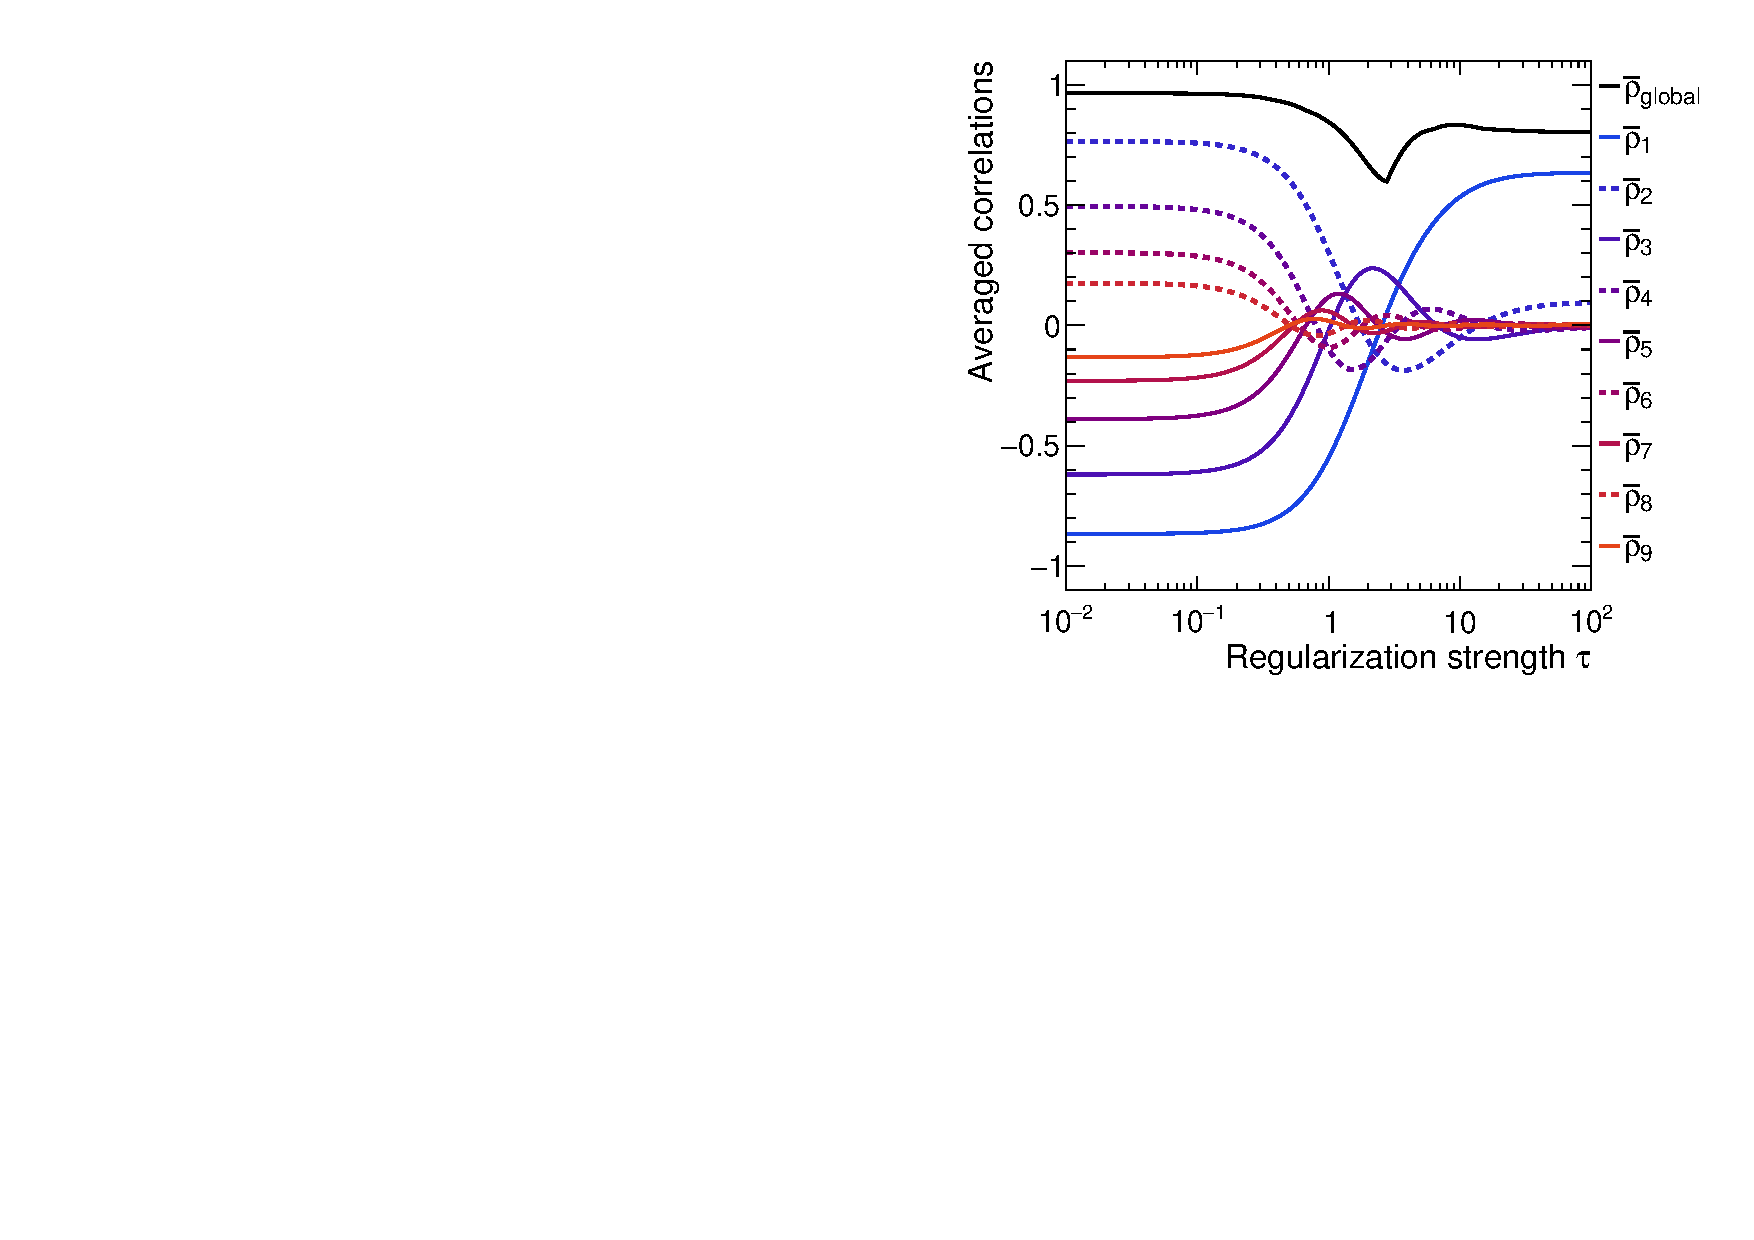
\includegraphics[width=0.48\textwidth]{figures/technique/scanTau.pdf}}\hspace{0.03\textwidth}
\subfloat[\label{fig:technique-tauscan-result}]{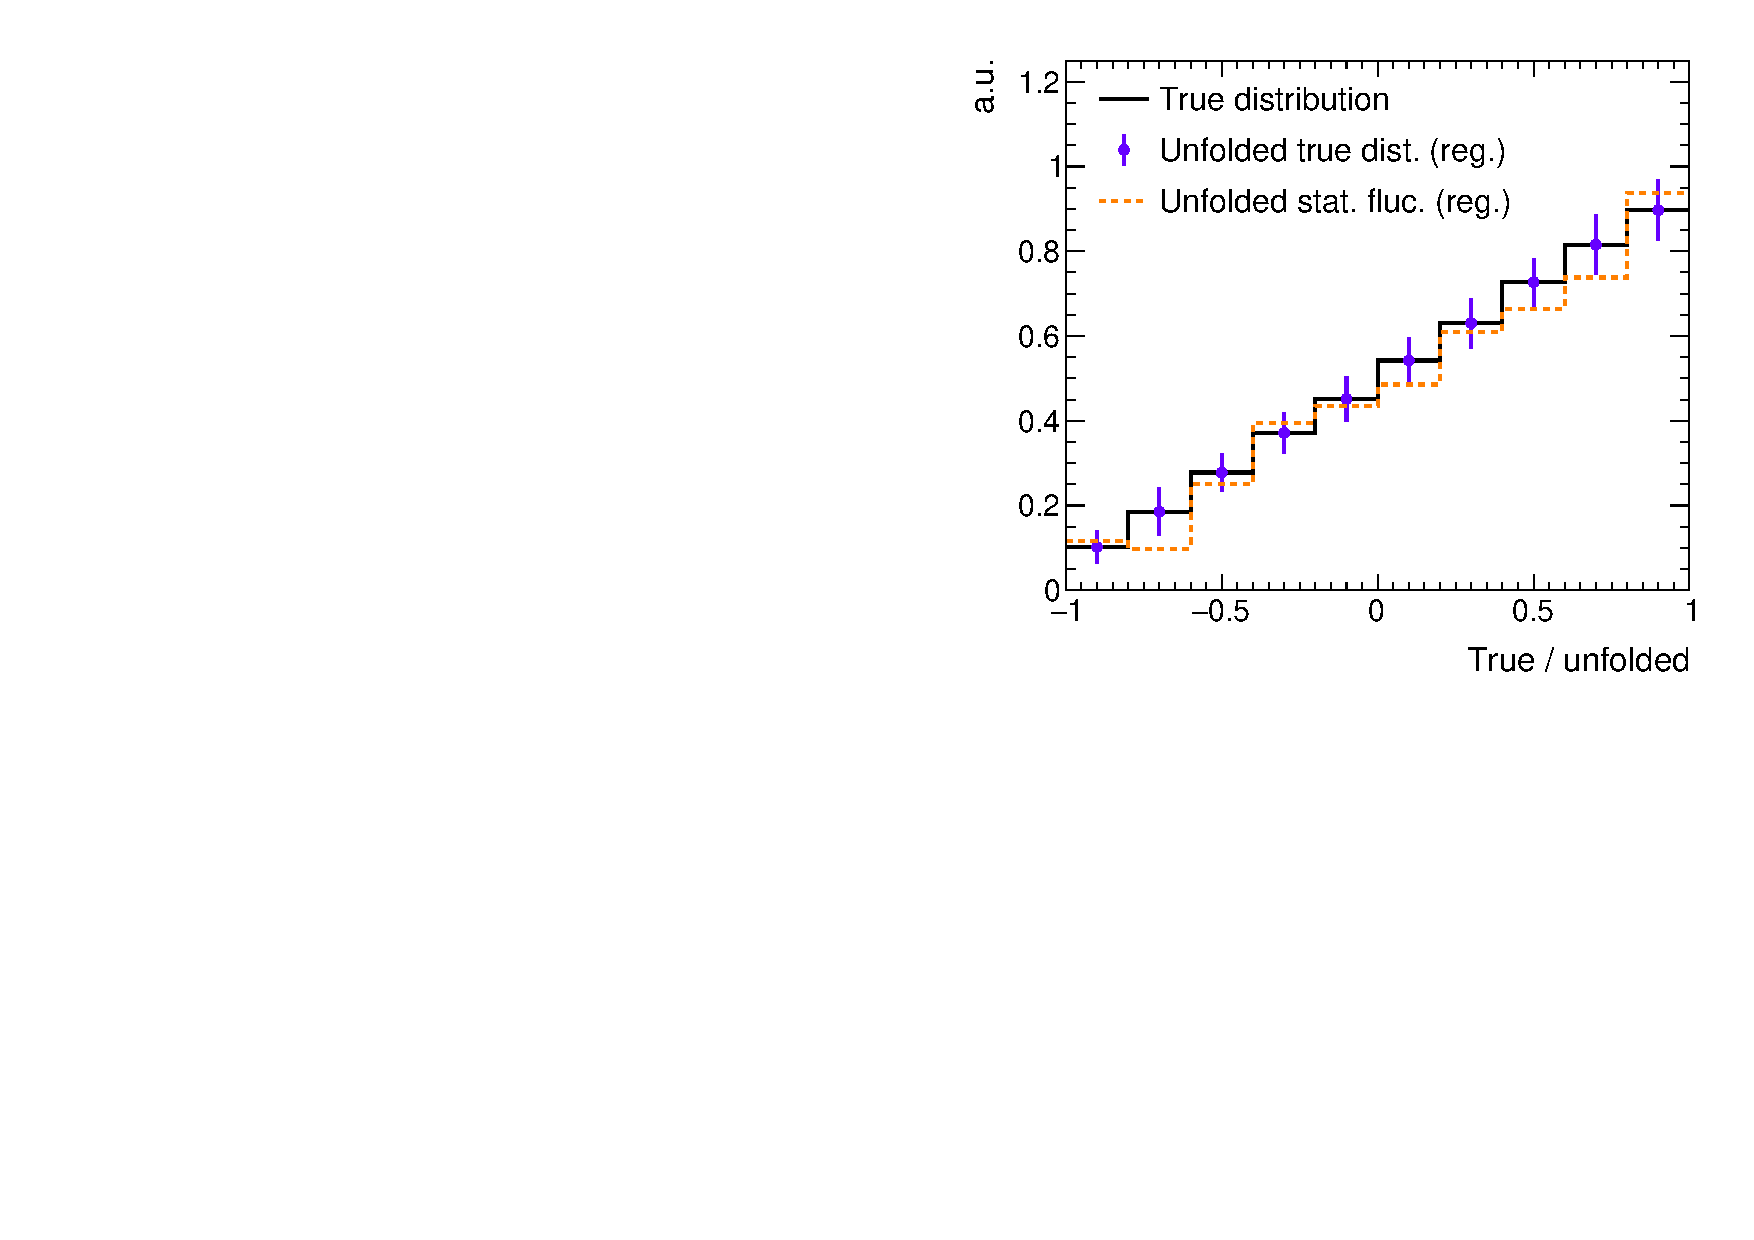
\includegraphics[width=0.48\textwidth]{figures/technique/unfoldDist.pdf}}
}

%\todo{show pulls for 1 bin in case of underregulariztion, overrgularization, optimal regularization}

In conclusion, unfolding is an ill-posed problem which requires regularization to obtain meaningful results that are stable against statistical fluctuations. The \TUNFOLD package regularizes the response matrix by suppressing solutions with large curvatures. However, this procedure induces bin-by-bin correlations as a function of the regularization strength. The correlations are kept small by adjusting the regularization strength to the minimum of the average global correlation coefficient.

